\chapter{Signal isolation: data reduction and uncertainty budget}
\label{c:SigIs}

\section*{Summary}
\label{s:SigIs:Summary}
In order to perform geophysical inversions on the static gravity field, a signal separation procedure is required, i.e.~the effect of an a-priori mass distribution must be removed, isolating an anomalous field \parencites[e.g.][]{Tenzer2009}{Tenzer2012refined}{Sjoberg2013}[][and references therein]{Aitken2015}.
The observed field stripped of the forward-modelled attraction of these ``known masses'' constitutes the input of inverse gravity modelling.
Any distribution of anomalous masses that results in the isolated field is a solution to the inverse problem.
Common reductions include the well-known terrain correction, i.e.~landmasses and bathymetry \parencites{Hinze2003}{Hinze2005}, which can be further refined by stripping the effect of subsurface density variations \parencite{Vajda2008}.

Uncertainties in the a-priori masses, such as unmodelled spatial variability in density, accumulate in the reductions and are propagated to the reduced data and to the inversion results.
Incomplete and inexact geological knowledge cannot be avoided, thus a perfect data reduction is unrealistic.
Therefore, an uncertainty-aware signal isolation process, i.e.~a process providing error estimates alongside its reduced gravity data, is a necessary step in estimating confidence of the inversion results, in statistical terms.
Error information is required in order to perform multi-observable integrated modelling \parencite[e.g.][]{Afonso2013}, comparisons \parencite[e.g.][]{Root2017}, or assimilation of geophysical models \parencites[e.g.~to assemble large scale maps from local studies, see][]{Tesauro2008}{Grad2009}{Molinari2011}.

The procedure and experiments described in this chapter were designed for local Moho inverse modelling, using global satellite-only gravity field models.
They were applied in the gravity-constrained thermal modelling strategy described in this thesis.
They include corrections for the terrain effect (topography, water, and ice), sediments and other intra-crustal density variations, and inhomogeneities in the lithospheric mantle.
Particular attention was paid to ensure spectral consistency between the forward-modelled reductions and the input gravity models.

Uncertainty was quantified through Monte Carlo error propagation \parencite{Aster2018}, resulting in a population of randomly perturbed reduction fields (according to a set of parameter uncertainty assumptions).
Results include the probability density function of these reductions, from which derived descriptive statistics was computed (e.g.~the spatial distribution of a defined confidence interval).

% The adjective ``anomalous'' is commonly used to indicate deviations from an a-priori reference. In order to prevent confusion with the strict-sense ``anomaly'', a gravity functional, in this section the term \textit{residual} is used to refer to any gravity data after the signal isolation procedure.

\section{Definition and computation of data reductions}
\label{s:SigIs:Defs}

\subsection{No-topography gravity disturbance}
\label{ss:SigIs:Defs:NETC}
In order to isolate the gravitational signal due to an unknown mass distribution, a technique known as ``stripping'' is employed \parencites{Vajda2008}{Tenzer2009}.
It consists in computing the gravitational effect of a ``known mass'' model, as inferred by other investigations, and removing it from the observed signal.
The gravimetric inverse problem is therefore formulated in terms of an anomalous gravity field resulting from the enquired mass/density distribution.

Following the recommendations in \textcite{Hackney2003} and \textcite{Vajda2007}, the formulation hereby presented is based on gravity disturbances, to avoid the ``Secondary Indirect Topographic Effect'' that arises when the topographic correction is applied to gravity anomalies.
Recalling the definition of gravity disturbance from \textcite{HofmannWellenhof2006}, section~2.12: it is defined as the difference in magnitude between the observed gravity vector $\bm{g}$ and the normal gravity vector $\bm{\gamma}$, at the same point $P$ of geocentric geodetic coordinates $(h, \lambda, \phi)$:
\begin{equation}
    \label{eq:red:GravDist}
    \delta g (h, \lambda, \phi) =
    \lvert \bm{g}(h, \lambda, \phi) \rvert -
    \lvert \bm{\gamma}(h, \lambda, \phi) \rvert
\end{equation}
where $\bm{g}$ is the gradient of the potential $\nabla W$ and $\bm{\gamma}$ is the gradient of the normal potential $\nabla U$.
By ``geocentric geodetic coordinates'' we refer to ``ellipsoidal coordinates'' \parencite{HofmannWellenhof2006}, with $h$ ellipsoidal height, $\phi$ geodetic latitude, and $\lambda$ geodetic longitude.
This follows from the definition of normal and disturbing potential, respectively $U$ and $T$:
\begin{equation}
    \label{eq:red:Pot}
    W(h, \lambda, \phi) = U(h, \phi) + T(h, \lambda, \phi)
\end{equation}
in which $W$ and $U$ can be decomposed in an attraction (gravitational) and a centrifugal component each, denoted with $\Phi$ \parencite[Eq.~5 and 13 in][]{Barthelmes2013}.
\begin{equation}
    \label{eq:red:PotAttr}
    \underbrace{W_{a}(h, \lambda, \phi) + \Phi(h, \phi)}_W =
    \underbrace{U_{a}(h, \phi) + \Phi(h, \phi)}_U +
    T(h, \lambda, \phi)
\end{equation}

To isolate the contribution of the anomalous density distribution we must remove the effect of a reference density model, against which anomalous densities are referred (in terms of density contrasts).
Following the strategy of \textcite{Vajda2006}, we can define a reference density model composed of two regions: one inside the reference ellipsoid, such as to generate the external normal potential, and one between the reference ellipsoid and the ``ellipsoidal topography'', i.e. the ``topography reckoned from the ellipsoid''.
As demonstrated by them, the gravity disturbance obtained by removing the effect of such a reference model is rigorously related with the ``gravitational attraction of the anomalous density distribution inside the entire Earth'' \parencite{Vajda2006}.
Omitting most of the derivation, for which I refer the reader to the contents in \textcite{Vajda2006}, I report here the following decomposition of the attraction potential $W_a$:
\begin{equation}
    \label{eq:red:Vdec1}
    W_a(h, \lambda, \phi) = V^{E}(h, \lambda, \phi) + V^{ET}(h, \lambda, \phi)
\end{equation}
where $V^{E}$ is the normal potential ($U_a$ in Eq.~\ref{eq:red:PotAttr}), due to the masses inside the reference ellipsoid, and $V^{ET}$ is the potential due to the masses between the ellipsoid and the topography.
Each of the potentials in Eq.~\ref{eq:red:Vdec1} is further decomposed, in the contribution of a reference density and in the contribution of the anomalous density distribution (in respect to the chosen reference). Therefore, omitting the position arguments ($h, \lambda, \phi$), the following is obtained:
\begin{equation}
    \label{eq:red:Vdec2}
    W_a = V_{R}^{E} + \delta V^{E} + V_{R}^{ET} + \delta V^{ET}
\end{equation}
where the terms with the subscript $R$ ($V_{R}^{E}$ and $V_{R}^{ET}$) denote the potentials due to the reference density contribution and the terms preceded by $\delta$ ($\delta V^{E}$ and $\delta V^{ET}$) denote the potentials due to the anomalous density contribution.
Recalling that $W_a - V_{R}^{E}$ (equivalent to $W_a - U_a$) is the disturbing potential $T$, Eq.~\ref{eq:red:Vdec2} can thus be rewritten as:
\begin{equation}
    \label{eq:red:DistT1}
    T = \left( \delta V^{E} + \delta V^{ET} \right) + V_{R}^{ET}
\end{equation}
The sum of $\delta V^{E}$ and $ \delta V^{ET}$ is the potential of the anomalous density distribution in the whole Earth $\delta V$, so the Eq.~\ref{eq:red:DistT1} can be further rearranged to:
\begin{equation}
    \label{eq:red:DistT2}
    T - V_{R}^{ET} = \delta V
\end{equation}

\Textcite{Vajda2006} proposed the notation $T^{NETC}$ for $T - V_{R}^{ET}$, the {NETC} acronym standing for ``No Ellipsoidal Topography of Constant density''.
Taking the vertical derivative of $T^{NETC}$ (applying the differential operator $-\partial / \partial h$, along the ellipsoidal normal), the ``NETC gravity disturbance'' is obtained:
\begin{equation}
    \label{eq:red:DistgNETC1}
    \delta_{g}^{NETC} =
    -\frac{\partial T^{NETC}}{\partial h} =
    -\frac{\partial \delta V}{\partial h} \equiv \delta A
\end{equation}
where $\delta A$ is the attraction of the anomalous density distribution.
The NETC gravity disturbance can be computed for each point gravity disturbance $\delta g$ using the following:
\begin{equation}
    \label{eq:red:DistgNETC2}
    \delta_{g}^{NETC} = \delta_{g} - A_{R}^{ET}
\end{equation}
here $A_{R}^{ET}$ is the forward-modelled attraction of the Earth topography of reference density.

The process that has been just described is conceptually akin to computing and removing a ``complete Bouguer correction'' \parencites{Hinze2003}{Mikuska2006} to gravity observations.
There are, however, some methodological discrepancies in the various definitions.
The method and terminology hereby presented should prevent confusion, providing a gravity quantity ($\delta_{g}^{NETC}$) which is formally related to the unmodelled density distribution, i.e. the component that was not accounted for in the reference model.

\subsection{Corrections to the gravity disturbance}
\label{ss:SigIs:Defs:Corrs}
Following the definitions used by \textcite{Vajda2008} and \textcite{Tenzer2009}, we classify the corrections to the gravity disturbance as topographic, bathymetric, and stripping.
They are fundamentally further refinements to the reference density model.
The topographic correction is computed with a reference density for both solid and liquid topography, i.e. for the strict sense topographic surface of land masses and for the surface of water bodies, both in respect to the reference ellipsoid.
The bathymetric correction consists in the removal of the effect of water density, expressed as contrast against the reference topographic density.
All further corrections (e.g. ice, sediments, crustal and mantle inhomogeneities...) go under the name of stripping -- they are computed as contrasts against reference, similarly to the bathymetric correction \parencite{Hammer1963}.

In regard to the masses below the reference ellipsoid, the reference densities are the ones of a model which results in the adopted normal potential, in concordance with the normal potential decomposition of Eq.~\ref{eq:red:Vdec1}.
A radially-stratified model of the interior, such as the PREM \parencite[Preliminary Reference Earth Model,][]{Dziewonski1981}, should satisfy this condition \parencite{Tscherning1981}.
Note that, in the adopted configuration, the `radial stratification' is actually defined by shells with a constant distance from the reference ellipsoid.

Stripping a set of \textit{known masses} (i.e. a-priori density distribution models) is often aimed at signal isolation.
For example, \textit{mantle gravity anomalies} \parencites[e.g.][]{Mooney2010}{Kaban2014} are obtained by stripping the ``crustal effect'', i.e. by correcting for a crust model \parencite[e.g. {CRUST1.0},][]{Laske2012Crust10}.
Starting from the NETC gravity disturbance introduced in the previous section (\ref{ss:SigIs:Defs:NETC}), corrections can be applied for ice, sediments, crustal heterogeneities.
The disturbance obtained after those corrections equals to a model Earth without topography above the ellipsoid and a reference-density (\textit{normal}) crust inside the ellipsoid, down to the crust-mantle interface.
In the unlikely case we had a perfect density model for these above-Moho masses, this reduced gravity would be equal to the attraction of anomalous densities in the mantle and core.

% discarding the following, shorter paragraph afterwards
% An application example is the work by \textcite{Tenzer2009}, who compiled and presented a set of global maps of the gravity disturbance --obtained from the EGM08 global gravity model \parencite{Pavlis2012EGM2008}-- corrected for the {CRUST2.0} model \parencite{Bassin2000Crust20} and for a reference crust of constant density.
% They chose the density of the latter in order to minimise the correlation between the crust-reduced disturbance and the Moho depth.
% By doing so, they obtained a global best-decorrelation density contrast of the ``consolidated crust'' (i.e. the bulk value) of \SI{-520}{\kilo \gram \per \metre \squared}, against the reference ellipsoid.
% This results in a stripped disturbance containing ideally no-topography, a \SI{3190}{\kilo \gram \per \metre \squared} crust between the ellipsoid surface and the Moho interface ($\num{2670} + \num{520}$), and the attraction of the density inhomogeneities below the Moho.
% It should be noted that there is no requirement of decorrelation between the crustal gravity signal and the one resulting from mantle inhomogeneities.

The work by \textcite{Tenzer2009} is an example of a similar application: they compiled and presented a set of global maps of the gravity disturbance (obtained from the EGM08 global gravity model, \cite{Pavlis2012EGM2008})-- corrected for the {CRUST2.0} model \parencite{Bassin2000Crust20}.
They also provided a crust reduction not depending on a-priori density models, using a decorrelation analysis between the crust--reduced disturbance and the Moho undulations.
A further development of that analysis is presented in \textcite{Tenzer2012contrast}.

\Textcite{Tenzer2009} also provided a global map of ellipsoid-- versus geoid--referenced topography and bathymetry corrected gravity disturbance.
Differences reach upwards to $\pm~14$~\si{\milli Gal} over continents, with a morphology highly correlated to geoidal undulations, as expected.

The methodology of \textcite{Tenzer2009} is the basis of the later work by \textcite{Tenzer2019}, which extended the forward modelling from {CRUST2.0} to {LITHO1.0} \parencite{Pasyanos2014}.

In crustal thickness modelling, signal isolation is obtained by concurrently correcting for above- and below-Moho masses ---as it has been done to obtain the global model {GEMMA} \parencites{Reguzzoni2013}{Reguzzoni2015}.
Most of global crustal density models are constrained by seismic data \parencites[e.g.][]{Laske2012Crust10}{Pasyanos2014}{Szwillus2019}, either completely or for the most part, and are constrained mainly in terms of velocity.
Reliance on assumed velocity-density conversions is therefore required.
Mantle stripping is affected by the same issues, and no ready-made velocity conversions of seismic models are available, as observed by \textcite{Tenzer2015}, requiring again to resort to conversion schemes \parencite[e.g.][]{Sebera2018}.
At mantle conditions, density conversion from velocity models \parencites[e.g.][]{Simmons2010}{Schaeffer2013} require modelling the concurring effect of temperature, pressure and composition on the elastic parameter --- which means carrying out comprehensive thermodynamic modelling \parencites{Connolly2005}{Connolly2009}.
These issues area dealt in detail in section~\ref{s:SigIs:InModels}.

The atmospheric correction has a range of \num{-0.04} to \SI{0.18}{\milli Gal} at the Earth surface \parencite{Tenzer2009_AtmCorr}.
Owing to its small value (3 orders of magnitude smaller than the effects of lithospheric mass inhomogeneities), it is often not considered for solid Earth signal isolation \parencite[e.g][]{Tenzer2019}.

\section{Forward modelling method}
\label{s:SigIs:Fwd}

\subsection{Spectral--domain forward modelling}
\label{ss:SigIs:Fwd:SHfwd}
Forward modelling the gravity field resulting from a mass distribution involves integrating its gravitational effects, thus evaluating the so called \textit{Newton integral} \parencite{HofmannWellenhof2006}:
\begin{equation}
    \label{eq:SHfwd:NewtonInt}
    W = G \iiint_v \frac{\rho}{r}dv
\end{equation}
where $G$ is the gravitational constant and $r$ is the distance from an element of mass of volume $v$, with $dm = \rho dv$.

Common methods to do so are either \textit{spatial--domain} or \textit{spectral--domain} forward modelling methods \parencite{Kuhn2005}.

In spatial--domain methods, the direct integration of masses is computed: volumes are decomposed (\textit{discretised}) in elementary bodies for which a solution to the Newton integral exists.
There are analytical formulas available for special cases (e.g. point masses, prisms \cites{Nagy2000}{Nagy2002}, or polyhedra \cites{Tsoulis2012}{Benedek2016}), while numerical approximations are more commonly employed for general solutions \parencites[e.g. spherical tesseroids][]{Heck2006}{Uieda2016}.
Numerical methods, in addition, are less time consuming in equivalent cases, e.g. by resorting to FFT, Taylor series expansion, or Gauss--Legendre cubature \parencite[see][and references therein]{Grombein2013}.
\nocite{Benedek2009} % also citing Benedek PhD thesis

Spectral--domain forward modelling, on the other hand, is based on the spherical harmonic (SH) series expansion of the Newtonian kernel \parencites{Rummel1988}{Blakely1996}{Root2015}{Wieczorek2007}.
In methods of this kind, coefficients of the resulting potential (or its derived functionals) are obtained from the mass distribution.
To assure convergence of the SH series, modelling is typically performed outside the \textit{Brillouin sphere}, i.e. a sphere encompassing all the field-generating mass, concentric with the spherical coordinate system \parencite{Moritz1980}.
Spectral--domain methods are commonly adopted for global computations, where they are considered less time consuming than spatial--domain methods, at least for degrees less than about 1000 \parencite{Kuhn2005}.
Computing higher maximum degrees of the SH series expansion, points inside the Brillouin sphere, and rugged topography are three factors that influence issues of numerical accuracy and divergence of spectral forward modelling methods \parencites{Hu2015}{Hirt2017}.
Combined spectral/spatial methods have been recently employed with success to obtain very high resolution synthetic gravity models \parencite{Hirt2019}.

The experiments described in this chapter were designed by taking into account the highest resolution available from satellite-only global gravity models -- which defined the maximum degree -- and the comparable (albeit lower) resolution of global density models to compute reductions (as described in the following section~\ref{s:SigIs:InModels}).
In addition, error assessment through random perturbation of the input models, the aforementioned Monte Carlo uncertainty propagation technique (described in section~\ref{s:SigIs:Impl}), requires a large number of forward iterations.
Therefore, I resorted to spectral--domain methods, using the method by \textcite{Wieczorek2007}, as implemented in the SHTOOLS code \parencite{Wieczorek2018}.

\Textcite{Wieczorek2007} provides a method for calculating the potential due to the topography, using a technique analogous to the cartesian (``flat-Earth'') method by \textcite{Parker1973}.
For its detailed description, I refer to the derivation of Eq.~6--12 in \textcite{Wieczorek1998}.
It is similar to a wider family of spherical-harmonics based solution to the volume integral, based on the binomial series expansion method, which \textcite{Root2015} defined as ``Fast Spectral Methods'' (FSMs).

Consider the case with a relief $h(\lambda, \theta)$ ($\theta = \SI{90}{\degree} - \phi$, colatitude), referenced to a spherical interface of radius $D$, with density $\rho(\lambda, \theta)$ radially constant between $h$ and $D$, $\rho$ considered negative when $h<0$.
Expressing the potential $W$ at a reference radius $R_0$ as a sum of spherical harmonic functions, we get:
\begin{equation}
    \label{eq:SHfwd:pot}
    W(r, \lambda, \theta) =
    \frac{GM}{r}
    \sum_{l=0}^{l_{max}}
    \sum_{m=-l}^{l}
    \left( \frac{R_0}{r} \right)^l
    C_{lm} Y_{lm} (\lambda, \theta)
\end{equation}
where $G$ is the gravitational constant, $M$ the total mass, $r$ calculation radius, and $Y_{lm}$ denotes the real spherical harmonics:
\begin{equation}
    \label{eq:SHfwd:rsh}
    Y_{lm}(\lambda, \theta) =
    \begin{cases}
        \overline{P}_{lm} (cos \theta) \cos m \lambda & \mbox{if } m \ge 0 \\
        \overline{P}_{l|m|} (cos \theta) sin |m| \lambda & \mbox{if } m < 0
    \end{cases}
\end{equation}
with $P_{lm}$ the normalized associated Legendre polynomials, omitted here.
Note that this notation, which is the one that \textcite{Wieczorek2007} adopted, differs from the one more commonly used in geodesy and geophysics \parencite[e.g.][]{HofmannWellenhof2006}.
Here, the order-wise sum over $m$ (the innermost sum) is performed starting from $-l$.
This results in a more compact notation: the spherical harmonics coefficients are denoted only by $C_{lm}$, instead of the usual ``$C_{lm}$'' and ``$S_{lm}$''.
As defined by the two cases of Eq.~\ref{eq:SHfwd:rsh}, positive-order coefficients would be usually noted with $C_{lm}$ and negative-order ones would be usually noted with $S_{lm}$.

Therefore, the formula for $C_{lm}$, on which the forward modelling of the relief is based, can be expressed in this form \parencite{Wieczorek2007}:
\begin{equation}
    \label{eq:SHfwd:coeffs}
    C_{lm} =
    \frac{4 \pi D^3}{M(2l+1)}
    \sum_{n=1}^{l+3}
    \frac{(\rho h^n)_{lm}}{D^n \ n!}
    \frac{\prod_{j=1}^{n}(l+4-j)}{(l+3)}
\end{equation}
where the $(\rho h^n)_{lm}$ denotes the spherical harmonics of the relief times density, obtained from:
\begin{equation}
    \label{eq:SHfwd:reliefSH}
    (\rho h^n)_{lm} =
    \frac{1}{4 \pi}
    \int_{\lambda, \theta}
    \left[ \rho(\lambda, \theta) h^n(\lambda, \theta) \right]
    Y_{lm}(\lambda, \theta) d(\lambda, \theta)
\end{equation}

Eq.~\ref{eq:SHfwd:coeffs} includes a Taylor series expansion of the power of the relief $(\rho h^n)_{lm}$.
If the sum is carried out up to its upper bound of the sum, $l+3$, it provides an exact solution.
However, the number of terms grows linearly with $l$.
Therefore, a truncation value $n_{max}$ is typically chosen, under the assumption that higher terms become more and more smaller \parencite{Wieczorek2007}.

However, \textcite{Balmino2012} and \textcite{Hirt2017} found that when a certain degree is reached, ``the energy of succeeding terms is larger than of the previous''.
They found this phenomenon to become significant around degree \num{1000} ---way above this experiment objective, which is limited by the maximum degree of satellite-only potential models (less than \num{300} as of March~2019).

The convergence of expansions of this kind has been rigorously studied by \textcite{Sun2001}, among others.
For a maximum degree $l = \num{360}$, a $n_{max}$ of \num{2} was shown to already provide less than \SI{1}{\percent} error ---in the case of topography.
Large deviations from the reference radius (e.g. in modelling deep and/or thick layers) may result in convergence problems, which can be mitigated by reducing the reference radius accordingly, as was shown later by \textcite{Root2015}.
For this reason, the experiments described in this section included a test against a spatial--domain benchmark.
It is described in more detail in section \ref{ss:SigIs:Fwd:LayerFwd}.

\Textcite{Wieczorek2007} notes that the potential (Eq.~\ref{eq:SHfwd:pot}) so obtained is valid only at $r > (D + h)$, i.e. outside the maximum radius of the relief ---this arises from the derivation of Eq.~\ref{eq:SHfwd:coeffs}, which is omitted here.

% accenno a ellipsoidal harmonics?
% trascurate qui - ne do il motivo?
% \Parencites{Claessens2013}{Rexer2016}

\subsection{Layer--wise modelling}
\label{ss:SigIs:Fwd:LayerFwd}
The forward modelling method by \textcite{Wieczorek2007}, which was just described in section~\ref{ss:SigIs:Fwd:SHfwd}, provides the potential due to relief against a reference sphere.
In order to model the gravity effect of a \textit{layer}, I devised a strategy based on superposition of two relief-against-sphere potentials, which is described hereafter.
Defining a \textit{layer} as a volume of radially constant density $\rho(\lambda, \phi)$, bound by two surfaces expressed by geocentric radii $t(\lambda, \phi)$ and $b(\lambda, \phi)$, respectively top and bottom, its resulting potential ($W_{b}^{t}$) is equal to the following difference:
\begin{equation}
    \label{eq:layerFWD:layerPot}
    W_{b}^{t} = W_{b}^{D} - W_{top}^{D}
\end{equation}
where subscripts denote the bottom boundary, superscripts denote the top boundary and $D$ is the radius of the reference sphere (from Eq.~\ref{eq:SHfwd:coeffs}).
Therefore, the potential of a layer with two arbitrary bounding surfaces can be forward modelled by computing the difference between two reliefs referred to the same sphere, $W_{b}^{D}$ and $W_{t}^{D}$.
A graphical representation of this difference is shown in Fig.~\ref{fig:SigIs:LayerDifference}.

\begin{figure}
    \begin{adjustbox}{center}
    \fbox{
        \begin{overpic}[width=\textwidth]{SH_layer_superposition_out.pdf}
            \put (15,4) {\huge$W_{b}^{D}$}
            \put (45,4) {\huge$W_{t}^{D}$}
            \put (75,4) {\huge$W_{b}^{t}$}
        \end{overpic}
    }
    \end{adjustbox}
    \caption[Sketch for the potential of a layer.]{
        Sketch for the potential of a layer bounded by surfaces $b$ and $t$, as expressed in Eq.~\ref{eq:layerFWD:layerPot}.}
    \label{fig:SigIs:LayerDifference}
\end{figure}

A pitfall of this strategy is that Eq.~\ref{eq:SHfwd:pot} needs to be evaluated twice, including the series expansion of Eq.~\ref{eq:SHfwd:coeffs}.
Other strategies with a similar aim have been developed \parencite[e.g.][]{Novak2006} and avoid this issue.
Nevertheless, the implementation by \textcite{Wieczorek2018} was preferred here, since it could be readily integrated in the random modelling scheme --- their Fortran functions are provided as {F2PY}--wrapped Python modules \parencite{Peterson2009}.

A potential source of issues is the depth of the modelled mass distribution, in terms of distance from the reference sphere: we are not in the same conditions that topographic effect modelling operates in.
\Textcite{Sun2001}, assessing the convergence issues of spherical harmonics methods based on the binomial expansion, observed that isostatic studies require much higher truncation numbers than terrain forward modelling.
They argued that this arises due to the much larger differences between isostatic roots and the compensation depth (e.g. \SI{100}{\kilo \metre}), compared to topography and the reference radius (about \SI{9}{\kilo \metre} of maximum topography).
This issue was also addressed by \textcite{Root2015}, who proposed an improved \textit{fast spectral method} \parencites{Rummel1988}{Novak2006} in order to model crustal and upper mantle regions.
They devised an ``error mitigation strategy'' which consists in lowering the reference sphere to model the deeper layers.
By doing so, they obtain results inside a $\pm$~\SI{4}{\milli Gal} difference range from spatial--domain forward modelling.

Compared with the mean Earth radius ($R = \SI{6371}{\kilo \metre}$), a \SI{40}{\kilo \metre} deep crust--mantle boundary accounts for about 6 thousands of $R$.
When modelling the underlying lithospheric mantle, a \SI{300}{\kilo \metre} lithosphere--asthenosphere boundary reaches about \SI{4.7}{\percent} of $R$.
This means that the layers modelled in the following experiments are likely to incur in the issues that have been just described.
Therefore. $D$ has been lowered accordingly for each modelled layer, setting it at the shallowest modelled depth.

Care must be paid to the sign of density, which is provided on the same grid as the top and bottom boundaries.
The relief-times-density product ($\rho h$ in Eq.~\ref{eq:SHfwd:reliefSH}) is negative for reliefs below the reference sphere (radius $D$).
Since in this setup all the boundary surfaces lie at radii less than $D$, by design, we must reverse the sign of the input density map.

\subsection{Spectral domain transform}
\label{ss:SigIs:Fwd:SHtransform}

Transforming a generic function $f$ in its spherical harmonic coefficients $f_{lm}$ goes under the name of Global Spherical Harmonic Analysis, GSHA \parencite{Sneeuw1994}.
It implies performing the following integration \parencite[Eq.~8 in][]{Wieczorek2007}:
\begin{equation}
    \label{eq:GSHA}
    f_{lm} =
    \frac{1}{4 \pi}
    \int_{\lambda, \theta}
    f(\lambda, \theta)
    Y_{lm}(\lambda, \theta) d(\lambda, \theta)
\end{equation}
which was already presented in Eq.~\ref{eq:SHfwd:reliefSH}, for the specific case of the relief-density product.
When $f$ is provided as a grid of discrete points, the integral of Eq.~\ref{eq:GSHA} can be evaluated numerically.
For these tests we utilised $n \times 2n$ grids (expressed as latitude times longitude) compliant to \textcite{Driscoll1994} sampling theorem.
Grids of this kind are also known as ``equally spaced''.
For such grids, the numerical solution to Eq.~\ref{eq:GSHA} is obtained through along--latitude FFT first, then by integration over longitude for each degree and order \parencites{Sneeuw1994}{Wieczorek2007}.
The transform on a $n \times 2n$ \textcite{Driscoll1994} grid is exact if $f$ is bandlimited to a maximum degree of $n/2 - 1$.

\subsection{Power spectrum and correlations between functions}
\label{ss:SigIs:Fwd:Spectrum}

For the degree $l$ of spherical harmonic coefficients $f_{lm}$, the \textit{degree variance} is defined as:
\begin{equation}
    \label{eq:DegVar}
    S_{ff}(l) = \sum_{m=-l}^{l} f_{lm}^2
\end{equation}
The degree variances spectrum, $S_{ff}(\bm{l})$ with $\bm{l} = (1, \dots, l_{max})$, provides a metric of the average power per harmonic degree \parencites{Rapp1982}{Wieczorek2007}{Hirt2015}.

Comparison between the coefficients of two functions, $f_{lm}$ and $g_{lm}$ may be performed by computing their cross-correlation:
\begin{equation}
    \label{eq:DegVarCross}
    S_{fg}(l) = \sum_{m=-l}^{l} \left( f_{lm} \enskip g_{lm} \right)
\end{equation}
which is usually expressed in a normalised form \parencites[e.g.][]{Phillips1980}{Rapp1982}{Rexer2016}, multiplying it with the factor \sloppy{${[S_{ff}(l) \cdot S_{gg}(l)]^{-\frac{1}{2}}}$}.
Note that while Eq.~12 in \textcite{Wieczorek2007} omits it, this normalisation factor is applied by the \textit{SHAdmitCorr} routine in {SHTOOLS} \parencite{Wieczorek2018}.

\section{Input mass distribution models}
\label{s:SigIs:InModels}

\subsection{Terrain correction}
\label{ss:SigIs:InModels:TC}
To model the solid topography, bathymetry (ocean, lakes) and ice, I adopted the {Earth2014} model \parencite{Hirt2015}.
It comprises data from SRTM (SRTM~v4.1 continental topography by \cite{Jarvis2008_SRTM4}, SRTM30~PLUS~v9 bathymetry by \cite{Becker_SRTM30plus}), Bedmap2 \parencite{Fretwell2013_Bedmap}, and GBT~v3 \parencite{Bamber2013_GBT}.
It is the base of the extensively used \verb|dV_ELL_Earth2014| topographic potential model \parencite{Rexer2016}.
In order to model an ellipsoid--referenced terrain correction (NETC, as described in section~\ref{ss:SigIs:Defs:NETC}) and to keep consistency with the subsurface stripping corrections applied afterwards, the already available potential model was not used.
Instead, I forward modelled an ad-hoc topographic potential, using the {Earth2014} shape model (i.e. relief provided as geocentric radii) as input.

% In addition to the spatial--domain comparison tests, shown in the supplementary section~\ref{s:SigIs:Test}, the terrain correction proved an useful benchmark for troubleshooting the method implementation: it could be readily compared with other topographic model, which would have likely been more difficult with subsurface correction models.
Uncertainty propagation on the terrain correction was not among the objectives of these experiments, therefore it was not carried out.
However, this ad-hoc modelling setup would enable to do so easily, e.g. if required in further developments.

\begin{figure}
    \begin{adjustbox}{center}
    \fbox{
        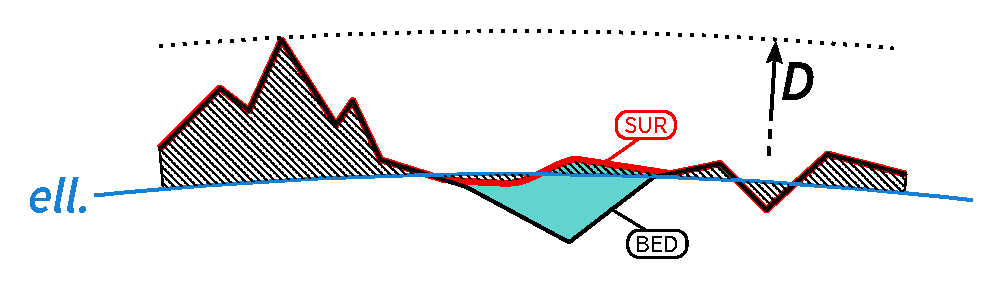
\includegraphics[width=\textwidth]{forward_scheme_topo_water_out.pdf}
    }
    \end{adjustbox}
    \caption[Terrain correction: sketch of the solid topography and ocean bathymetry stripping.]{
        Terrain correction: sketch of the solid topography and ocean bathymetry stripping.
        The hatched area 
            
\includegraphics[width=0.5\baselineskip]{symbol_hatched_out.pdf}
        covers the layer--volume of solid topography, between the reference ellipsoid (\textit{ell.}) and the \texttt{SUR} surface.
        The teal-coloured area 
            
\includegraphics[width=0.5\baselineskip]{symbol_water_out.pdf}
        represents the layer--volume of ocean bathymetry stripping, between the \texttt{BED} and \texttt{SUR} surfaces. Note that \texttt{SUR} and \texttt{BED} coincide onshore.
        $D$:~reference radius.
        For a description of surfaces, see Tab.~\ref{tab:E2014fwdSurfaces}.
    }
    \label{fig:E2014fwdLayersSketch}
\end{figure}

Potential forward modelling of the {Earth2014} relief grids was partitioned in solid topography, ocean bathymetry, lake bathymetry, on-shore ice, off-shore ice, and on-lakes ice.
Each unit was modelled as a distinct layer, with its own forward modelling call.
\textit{Solid topography} is defined by the \verb|SUR| surface, the topmost surface in {Earth2014}, which includes the top surface of ice masses and of all bodies of water.
The layers are summarised in Tab.~\ref{tab:E2014fwdLayers}, along with their densities and the defining top and bottom surfaces.
The general scheme of layers arrangement is sketched in Fig.~\ref{fig:E2014fwdLayersSketch}, showing the modelling of solid topography and ocean stripping as an example.

The boundary surfaces extracted from {Earth2014} data are described in Tab.~\ref{tab:E2014fwdSurfaces}.
Discrimination between ocean and lake bathymetry, and between on-shore and off-shore ice was performed using the ``mask grid files'' provided with the model, which include land types flags.

In order to obtain an exact number of samples nodes along latitude and longitude, all the grids were resampled to a \SI{0.08}{\degree}~by~\SI{0.08}{\degree} equally spaced grid ($n \times 2n$, as described in section~\ref{ss:SigIs:Fwd:SHtransform}), using a modified Akima piecewise cubic Hermite interpolation---a Matlab--specific implementation of \textcite{Akima1974}---which successfully avoided local artefacts and overshoots.
The original grids in \textcite{Hirt2015} are provided with a \SI{1}{min} and \SI{5}{min} spacing, the latter being a box--mean downsampled version of the former.
To ease the computational requirements, the \SI{5}{min} version was used here, justified by the much lower target resolution of our terrain forward model ($l_{max} = \num{280}$, resulting in a half--wavelength resolution of about \SI{0,64}{\degree})
This resulted in slight upsampling, from \SI{5}{min} (equal to \SI[parse-numbers=false]{0.08\overline{3}}{\degree}) to \SI{0.08}{\degree}.

The \textit{complete terrain correction} was then computed by summing the gravity effect of all the forward modelled masses.
Expressed in terms of correction to the gravity disturbance (the \textit{attraction of the Earth topography} $A_{R}^{ET}$ in Eq.~\ref{eq:red:DistgNETC2}), it results in the following:
\begin{multline}
    \label{eq:CompleteTC}
    A_{R}^{ET} =
    -\frac{\partial}{\partial h}
    (
        W^{\mathtt{SUR}}_{\mathtt{GRS80}} +
        W^{\mathtt{SUR}}_{\mathtt{BED\_OCEANS}} +
        W^{\mathtt{SUR}}_{\mathtt{BED\_LAKES}} + \\
        + W^{\mathtt{TBI}}_{\mathtt{ICEbot\_onshore}} +
        W^{\mathtt{TBI}}_{\mathtt{ICEbot\_offshore}} +
        W^{\mathtt{TBI}}_{\mathtt{ICEbot\_onlakes}}
    )
\end{multline}
in which the terms refer to the labels in Tab.~\ref{tab:E2014fwdLayers}.

\begin{table}[ht]
    \caption[Terrain correction scheme: summary of the layers and their defining surfaces and densities.]{
        Terrain correction scheme: summary of the layers and their defining surfaces and densities.
        \textit{Layer:}~density of the modelled mass.
        \textit{Ref.:}~reference density for stripping corrections.
        \textit{Contrast.:}~layer density minus reference density.
        \texttt{GRS80}: GRS80 ellipsoid in geocentric radius \parencites{Moritz1980_GRS80}{Moritz2000_GRS80}. For a description of surfaces, see Tab.~\ref{tab:E2014fwdSurfaces}.}
    \begin{adjustbox}{center}
        % E2014fwdLayers table
\begin{tabular}{lllrrr}
    \toprule   
    {} & \multicolumn{2}{c}{\textbf{Boundary surfaces}}  & \multicolumn{3}{c}{\textbf{Density [\si{\kilo \gram \per \cubic \metre}]}}\\
        \cmidrule{2-3}
        \cmidrule{4-6}
        \textbf{Layer name} & \multicolumn{1}{c}{\textbf{Top}} & \multicolumn{1}{c}{\textbf{Bottom}} & Layer & Ref. & Contrast \\
    \midrule
    Solid topography &
    \texttt{SUR} & \texttt{GRS80} &
    \num{2670} & & \\

    \textit{Stripping of} & & & & \\

    \quad ocean bathymetry &
    \texttt{SUR} & \texttt{BED\_OCEANS} &
    \num{1030} & \num{2670} & \num{-1640} \\

    \quad lake bathymetry &
    \texttt{SUR} & \texttt{BED\_LAKES} &
    \num{1000} & \num{2670} & \num{-1670} \\

    \quad on-shore ice &
    \texttt{TBI} & \texttt{ICEbot\_onshore} &
    \num{915} & \num{2670} & \num{-1755} \\

    \quad off-shore ice &
    \texttt{TBI} & \texttt{ICEbot\_offshore} &
    \num{915} & \num{1030} & \num{-1755} \\

    \quad on-lakes ice &
    \texttt{TBI} & \texttt{ICEbot\_onlakes} &
    \num{915} & \num{1000} & \num{-1755} \\
    \bottomrule
\end{tabular}
    \end{adjustbox}
    \label{tab:E2014fwdLayers}
\end{table}

\begin{table}[ht]
    \caption[Description of the input surfaces utilised in the terrain correction, as extracted from {Earth2014}.]{
        Description of the input surfaces utilised in the terrain correction, as extracted from {Earth2014}. Text between quotes is from Table~1 in \textcite{Hirt2015}. Land type flag description from the {Earth2014} \textit{readme} file \parencite{Hirt2015_Earth2014readme}.}
    \begin{adjustbox}{center}
        % E2014fwdSurfaces table
\begingroup\setlength{\fboxsep}{0pt}
\colorbox{tablebackground}{%
\begin{tabular}{lp{0.7\textwidth}}
    \toprule   
    \textbf{Surface} & \textbf{Description} \\
    \midrule
    \texttt{SUR} &
    ``Lower interface of the atmosphere'' i.e.~surface of the continental topography, lakes, oceans and ice sheets. \\
    & Unmodified from Earth2014 data. \\
    \texttt{BED\_OCEANS} &
    ``Bedrock, planet without water and ice'' masked by land type flag equal to 2 (ocean bathymetry). \\
    \texttt{BED\_LAKES} &
    ``Bedrock, planet without water and ice'' masked by land type flag equal to 3, 4 (inland lakes) or 8 (ice covered lake). \\
    \texttt{TBI} &
    Topography, including ice, without liquid water. \\
    & Unmodified from Earth2014 data. \\
    \texttt{ICEbot\_onshore} &
    \texttt{TBI} minus ice thickness, masked by land type flag equal to 5 and 6 (ice cover). \\
    \texttt{ICEbot\_offshore} &
    \texttt{TBI} minus ice thickness, masked by land type flag equal to 7 (ice shelf).  \\
    \texttt{ICEbot\_onlakes} &
    \texttt{TBI} minus ice thickness, masked by land type flag equal to 8 (ice covered lake).  \\
    \bottomrule
\end{tabular}
}\endgroup

    \end{adjustbox}
    \label{tab:E2014fwdSurfaces}
\end{table}

\begin{figure}
    \begin{adjustbox}{center}
        \fbox{
            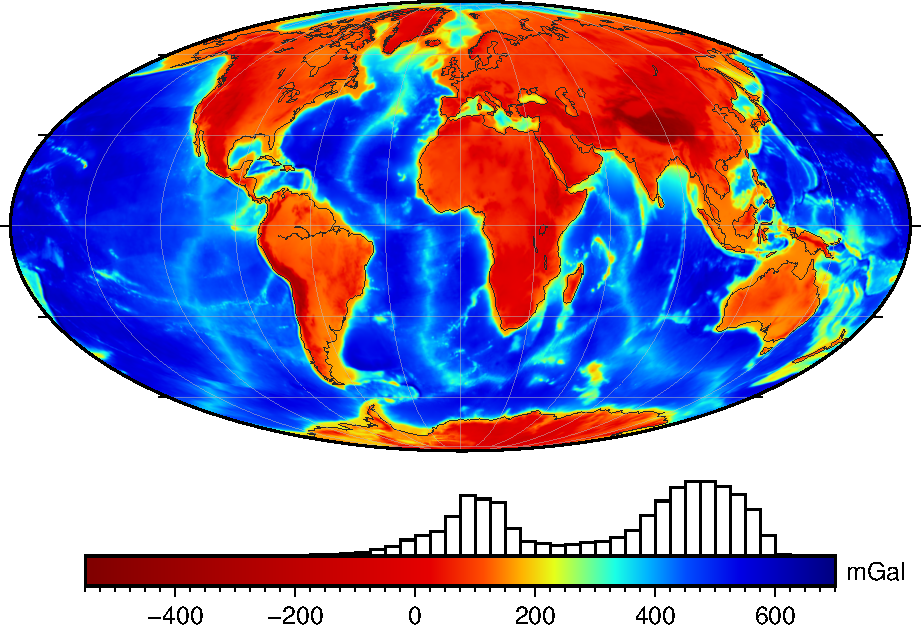
\includegraphics[width=\textwidth]{maps/sig_isol/TC_g_rad_HD_LP.pdf}
        }
    \end{adjustbox}
    \caption[Radial component of the terrain correction, corrections included.]{Radial component of the terrain correction, corrections included. It is expressed as positive upwards (i.e. the attraction of solid topography is negative). The histogram over the colour scale is equal-area normalised, using a spherical approximation.}
    \label{fig:E2014fwd_out_TC_g_rad}
\end{figure}

\subsection{Lithospheric density model}
\label{ss:SigIs:LITHOmodel}

These experiments rely on the {LITHO1.0} model by \textcite{Pasyanos2014}, which expands on the results of CRUST5.1 \parencite{Mooney1998_Crust51}, CRUST2.0 \parencite{Bassin2000Crust20} and CRUST1.0 \parencite{Laske2012Crust10}.
\Textcite{Pasyanos2014} provide a global model of the lithosphere, from the topography to the base of lithospheric mantle (lithosphere--asthenosphere boundary, LAB), parametrized vertically in a series of `geophysical layers'.
Horizontally, these layers are discretised on a icosahedron--based tessellation, which results in an average arc-distance of about \SI{1}{\degree} between points.
The following physical properties are provided in each of the layers, for each of the depth-columns defined by the model nodes: compressional wave velocity ($V_{P}$), shear wave velocity ($V_{S}$), and density ($\rho$).
In each node, the properties inside each layer are constant in the radial direction.

Thickness and properties of the crust and lithospheric mantle in {LITHO1.0} are the result of a targeted--grid--search based inversion of surface wave dispersion maps.
Their starting model is based on the data in {CRUST1.0} \parencite{Laske2012Crust10}, an updated version of the sediment model by \textcite{Laske1997_sediments}, an updated crustal thickness from undisclosed 1D seismic profiles (active source and receiver function studies), the lithospheric thickness by \textcite{Pasyanos2005}, the upper mantle velocity from {LLNL-G3Dv3} \parencite{Simmons2012_LLNL}, pure--gravity based crustal thickness in Antarctica \parencite{Block2009} and other locations lacking seismic data (undisclosed).
The lithospheric thickness in \textcite{Pasyanos2005} was in turn constrained by continental heat--flow based estimates by \textcite{Artemieva2006} and oceanic lithospheric cooling \parencite{Turcotte1982_geodynamics}.

\begin{table}
    \caption[Thickness and density of the layers from {LITHO1.0}.]{
        Average (\textbf{Avg.}) and standard deviation (\textbf{SD}) of thickness and density of the layers from {LITHO1.0} \parencite{Pasyanos2014}.
        {SEDS}:~sediments,
        {CRUST}:~crystalline crust (basement to Moho),
        {LID}:~lithospheric mantle (Moho to LAB).
        See Tab.~\ref{tab:LithoLayersGroups} for the statistics on aggregated layers.
        Note that strongly asymmetrical distributions result in standard deviations larger than the average value.
    }
    \begin{adjustbox}{center}
        % Litho1.0 used layers table
\begin{tabular}{lllllllll}
    \toprule
        & \multicolumn{2}{c}{\textbf{Average}\textsuperscript{*}} \\
        \cmidrule{2-3}
        & \multicolumn{1}{c}{\textbf{Thickness}} & \multicolumn{1}{c}{\textbf{Density}\textsuperscript{†}} \\
        \textbf{Layer} & \multicolumn{1}{c}{\textbf{[\si{\kilo \metre}]}} & \multicolumn{1}{c}{\textbf{[\si{\kilo \gram \per \cubic \metre}]}} &
        \multicolumn{6}{c}{\textbf{Cumulative averages}} \\
    \midrule

    SEDS 1 & \num{0.62}\textsuperscript{‡} & \num{1978} &
    \rdelim\}{3}{*} & \multirow{3}{*}{\shortstack[l]{
        \SI{1.13}{\kilo \metre}\textsuperscript{‡} \\ \SI{2128}{\kilo \gram \per \cubic \metre}}} &
    \rdelim\}{6}{*} & \multirow{6}{*}{\shortstack[l]{
        \SI{13.2}{\kilo \metre} \\ \SI{2827}{\kilo \gram \per \cubic \metre}}} &
    \rdelim\}{7}{*} & \multirow{7}{*}{\shortstack[l]{
        \SI{95.1}{\kilo \metre} \\ \SI{3213}{\kilo \gram \per \cubic \metre}}} \\
    SEDS 2 & \num{2.21}\textsuperscript{‡} & \num{2341} \\
    SEDS 3 & \num{3.10}\textsuperscript{‡} & \num{2558} \\

    CRUST 1 & \num{5.63} & \num{2719} &
    \rdelim\}{3}{*} & \multirow{3}{*}{\shortstack[l]{
        \SI{12.2}{\kilo \metre} \\ \SI{2856}{\kilo \gram \per \cubic \metre}}} \\
    CRUST 2 & \num{6.49} & \num{2820} \\
    CRUST 3 & \num{9.06} & \num{2966} \\

    LID & \num{81.9} & \num{3317} \\

    \bottomrule
    \multicolumn{9}{l}{\textsuperscript{*}\footnotesize{
        Weighted by the cosine of latitude of each grid node, to account for the convergence of meridians.}
    } \\
    \multicolumn{9}{l}{\textsuperscript{†}\footnotesize{
        Density average is also weighted by thickness.}
    } \\
    \multicolumn{9}{l}{\textsuperscript{‡}\footnotesize{
        Average of nodes with non-zero sediment thickness.}
    }
\end{tabular}

    \end{adjustbox}
    \label{tab:LithoLayers}
\end{table}

\begin{table}
    \caption[Thickness and density of grouped layers from {LITHO1.0}.]{
        Average and standard deviation of thickness and density of grouped layers from {LITHO1.0} \parencite{Pasyanos2014}. See Tab.~\ref{tab:LithoLayers} for the non aggregated layers and notes on computation. Standard deviations are shown in parentheses.
    }
    \begin{adjustbox}{center}
        % Litho1.0 used layers table
\begin{tabular}{lrcrcrc}
    \toprule
    \textbf{Layer} \\
    \midrule
    SEDS  1 &
    \rdelim\}{3}{*} & \multirow{3}{*}{\shortstack[c]{
        SEDS \\ 1.00~(1.56)~\si{\kilo \metre} \\ 2128~(182)~\si{\kilo \gram \per \cubic \metre}}} &
    \rdelim\}{6}{*} &  \multirow{6}{*}{\shortstack[c]{
        SEDS + CRUST \\ 22.1~(15.8)~\si{\kilo \metre} \\ 2827~(82)~\si{\kilo \gram \per \cubic \metre}}} &
    \rdelim\}{7}{*} &  \multirow{7}{*}{\shortstack[c]{
        whole lithosphere \\ 104.0~(67.7)~\si{\kilo \metre} \\ 3213~(91)~\si{\kilo \gram \per \cubic \metre}}} \\
    SEDS  2 \\
    SEDS  3 \\
    CRUST 1 &
    \rdelim\}{3}{*} &  \multirow{3}{*}{\shortstack[c]{
        CRUST \\ 21.2~(15.6)~\si{\kilo \metre} \\ 2856~(76)~\si{\kilo \gram \per \cubic \metre}}} \\
    CRUST 2 \\
    CRUST 3 \\
    LID     \\
    \bottomrule
\end{tabular}
    \end{adjustbox}
    \label{tab:LithoLayersGroups}
\end{table}

As the authors of {LITHO1.0} point out, it would be naive to assume that the model resolves the complicated lateral and vertical inhomogeneities of the lithosphere.
They aimed at ``a consistent, defensible, and updatable model that is compatible with observed data and can capture some of the geophysical community's collective understanding of the Earth'' \parencite{Pasyanos2014}.
In the context of these experiments, {LITHO1.0} provides a global, readily accessible model of density in sediments, crystalline crust, and lithospheric mantle.
It provides a model at a nominal resolution which is comparable with the resolving power of geophysical inversion based on satellite--only global gravity models.

Compiling the available data in a global model of the crust and/or lithosphere is still a challenging task, requiring the retrieval, harmonisation and gridding of a huge assortment of data sets.
The recent global crustal thickness by \textcite{Szwillus2019} was also considered as an alternative crustal model, due to two features that are particularly relevant for these data reduction experiments:
(1) the transparency in its construction, since the input data is disclosed and accessible \parencite{Mooney2015_globalcrust} and the methods are reproducible;
(2) the estimation of uncertainty is described and its grids are provided: they could be employed in a realistic error propagation scheme to the forward modelled gravity field.

Nevertheless, while {LITHO1.0} is lacking in those two aspects, it was still adopted as our reference density model, owing to:
(1) its integration with a global sediment thickness model;
(2) its seismic multi--observable nature, which takes advantage of the sensitivity to discontinuities of controlled--source and receiver functions, from prior models, and the sensitivity to ``bulk Earth properties'' ---from which density can be derived--- of surface waves;
(3) its relative independence from gravity data: aiming at preventing any circular reference (i.e. correcting gravity data with models which were inverted from gravity), full independence would be ideal. While {LITHO1.0} is not free from local gravity--based \textit{fill-ins} (Antarctica and other undisclosed locations), the inversion starting models and inversion strategy of \textcite{Pasyanos2014} is predominantly based on seismic data.
It is for this particular reason that multi--observable models that include global gravity models among their input data were left out, such as the recent \textit{LithoRef18} model \parencite{Afonso2019}.

In summary, {LITHO1.0} is a reasonable compromise model, fit for this methodological test, albeit affected by the aforementioned pitfalls.
It must be noted that the procedure hereby described could be easily scaled to different global models and to more refined uncertainty data, as further described in section~\ref{s:SigIs:Impl}.

The three properties provided in {LITHO1.0} ($V_P$, $V_S$, and $\rho$) are not independently estimated quantities: the starting model reflects the reference values and parameter relationships defined by the  ``primary crustal types'' and their variants, from {CRUST5.1} \parencite{Mooney1998_Crust51} and the following version (as mentioned above).
The $V_S/V_P$ ratio in the crust is unmodified from CRUST1.0 data.
The Poisson's ratio \parencite[see e.g.][]{Sheriff2002} in the lithospheric mantle, from which the $V_S/V_P$ can be derived, is fixed to \num{0.26}.
Density in the lithospheric mantle (``LID''~layer) is provided as a constant value (\SI{3300}{\kilo \gram \per \cubic \metre}).
The extraction of a velocity-converted density in the LID is the subject of the following section (\ref{ss:SigIs:InModels:SCLM}).

Regarding data uncertainty, no space--wise error information is provided, neither any information on data quality (e.g. distance to data or sources of the starting model).
These experiments therefore resorted to a simplified error model, which is described in section~\ref{s:SigIs:Impl}.

The water and ice layers were discarded, since {Earth2014} \parencite{Hirt2015} relies on updated and revised data.
Therefore, the top of the solid--Earth layers of {LITHO1.0} (starting from the first sedimentary layer) has been re-referenced to {Earth2014} bedrock (\texttt{BED} surface, see Tab.~\ref{tab:E2014fwdSurfaces} and \cite{Hirt2015_Earth2014readme}).

As already mentioned for the terrain correction, this data also needs to be gridded in a format compatible with the chosen gravity forward modelling: an equally spaced $n \times 2n$ grid, consistent with \textcite{Driscoll1994} sampling theorem.
Triangulation from the original tessellated data to geographic coordinates was performed using the {Stripy} package \parencites{Moresi2019}{Moresi2019_zenodo} and {litho1pt0} \parencite{Moresi2019_litho1pt0}, a Python interface to {LITHO1.0}.

\subsection{Velocity--density conversion in the lithospheric mantle}
\label{ss:SigIs:InModels:SCLM}

Density in {LITHO1.0} \parencite{Pasyanos2014} lithospheric mantle ({LID}~layer) is provided constant at \SI{3300}{\kilo \gram \per \cubic \metre}.
$V_P$ and $V_S$ are both provided, but with a Poisson ratio ($\sigma$) fixed at~\num{0.26}.
The $V_S / V_P$ ratio is directly related to $\sigma$ \parencite{Sheriff2002}:
\begin{equation}
    \label{eq:VSVP_PoissonRatio}
    \frac{V_S}{V_P} =
    \sqrt{\frac{0.5 - \sigma}{1 - \sigma}}
\end{equation}
This results in a $V_S / V_P$ ratio in {LITHO1.0} lithospheric mantle of about \num{0.57}.

Therefore, a velocity-to-density conversion was set up, based on assumptions on composition and thermodynamic modelling.
In order to define this strategy, a trade-off was needed between uniform velocity-density scaling (i.e. with a constant ratio) and detailed modelling of mineralogical phases, which goes beyond the scope of these experiments.

The basis for the conversion is the compositional model by \textcite{Griffin2009}.
As they argued, there is a broad relation between the lithospheric mantle composition and the tectonothermal age of the overlying crust.
Therefore, I have grouped the crustal types from {CRUST1.0} \parencite{Laske2012Crust10} in a simplified two-member model of LID composition.
The result of this partition is shown in Fig.~\ref{fig:SigIs:LithoAges}.
The two members are \textit{archon} (Arc\_1) and \textit{tecton} (Tc\_1), the code from \textcite{Griffin2009} shown in parentheses.
They represent a simplified but realistic discrimination between `young' (Phanerozoic) and `old' lithospheric mantle (e.g.~protons, shields, cratons).

\begin{figure}
    \begin{adjustbox}{center}
        \fbox{
            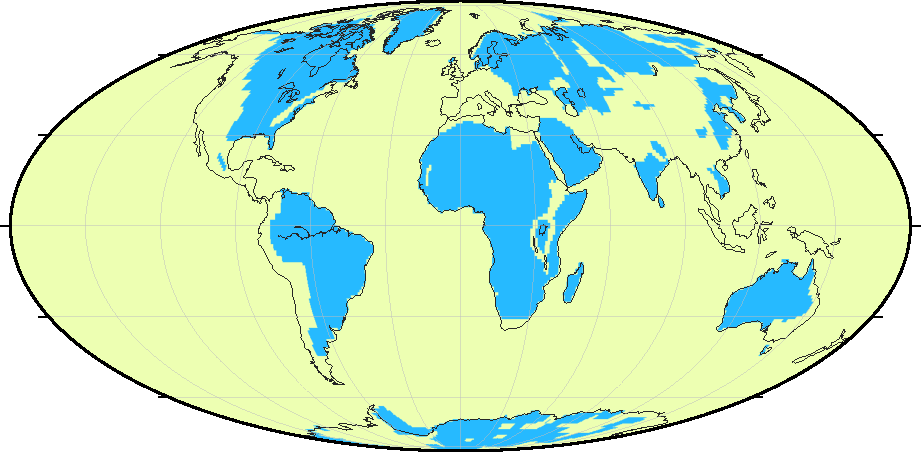
\includegraphics[width=\textwidth]{maps/sig_isol/CTypes_AT.pdf}
        }
    \end{adjustbox}
    \caption[Tectonothermal age partition of the lithospheric mantle.]{
        Two-member tectonothermal age partition of the lithospheric mantle, derived from the crustal types by \textcite{Laske2012Crust10}.
        \textbf{Light green}:~`young' lithosphere (Phanerozoic, with \textit{tecton} composition), \textbf{blue}:~`old' lithosphere (protons, shields, cratons, with \textit{archon} composition).
    }
    \label{fig:SigIs:LithoAges}
\end{figure}

Phase equilibria were modelled with the {Perple\_X} program \parencites{Connolly2005}{Connolly2009}, adopting the {hp02ver} thermodynamic data base \parencites{Powell1998_hp02}{Ghiorso2002_pMELTS}, which is a comprehensive chemical model for silicates in the lithosphere, appropriate for depths less than \SI{440}{\kilo \metre}.
I extracted $V_S$ and $\rho$ in the pressure range of interest (up to the maximum LAB depth, \SI{300}{\kilo \metre}) and then fitted a $\rho (P, V_S)$ linear interpolator on the data.
Pressure values were computed as purely lithostatic pressure, by depth-integration of the density of the overlying layers and of the constant \SI{3300}{\kilo \gram \per \cubic \metre} lithospheric mantle density (prior to conversion).
The conversion curves on the pressure-velocity field are shown in Fig.~\ref{fig:SigIs:VelConvCurves}.

\begin{figure}
    \begin{adjustbox}{center}
        \fbox{
            \begin{tabular}{cc}
                \begin{overpic}[
                    width=0.65\textwidth,
                    clip, trim=0.5cm 0.25cm 1.15cm 1cm
                    ]{VSconv/VSconv_arc.pdf}
                    \put (65,85) {\large \textsf{\textit{Archon}}}
                \end{overpic}
                \begin{overpic}[
                    width=0.65\textwidth,
                    clip, trim=0.5cm 0.25cm 1.15cm 1cm
                    ]{VSconv/VSconv_tec.pdf}
                    \put (65,85) {\large \textsf{\textit{Tecton}}}
                \end{overpic}
            \end{tabular}
        }
    \end{adjustbox}
    \caption[Pressure and shear wave velocity density conversion.]{Pressure and shear wave velocity ($V_S$) density conversion curves for the two-member lithospheric mantle composition model. Density is plotted with contours, the gray-filled area shows the bounds of the modelled domain.
    }
    \label{fig:SigIs:VelConvCurves}
\end{figure}

\begin{figure}
    \begin{adjustbox}{center}
        \fbox{
            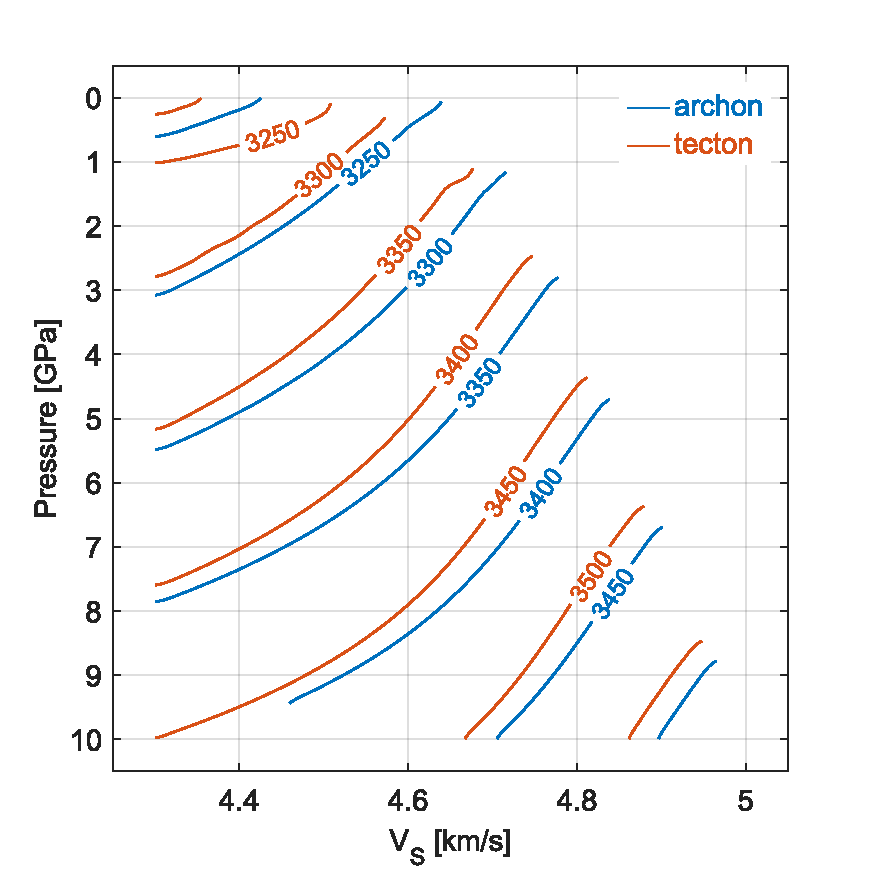
\includegraphics[
                width=0.65\textwidth,
                clip, trim=0.5cm 0cm 1.15cm 1cm
                ]{VSconv/VSconv_both_mod.pdf}
        }
    \end{adjustbox}
    \caption[Density conversion curves: direct comparison between the two members.]{
        The density conversion solutions for the two-member composition model (as shown in Fig.~\ref{fig:SigIs:VelConvCurves}), plotted overlaid on the same pressure-velocity field.
    }
    \label{fig:SigIs:VelConvCurves_comp}
\end{figure}

Since the whole lithospheric mantle is originally defined in bulk columns, Moho to LAB, it was sliced depth-wise prior to velocity conversion.
While $V_S$ does not change depth-wise, this allowed for a finer discretisation of pressure: inside each slice, the value at the slice midpoint was adopted.
This slicing operation follows the same depth discretisation that was adopted for the reference density model, as described in the next section~\ref{ss:SigIs:InModels:REF}.
Conversion results, condensed after slicing using a thickness-weighted average, are shown in Fig.~\ref{fig:SigIs:LID_VS-density_map}.

\begin{figure}
    \begin{adjustbox}{center}
        \fbox{
            \begin{tabular}{c}
                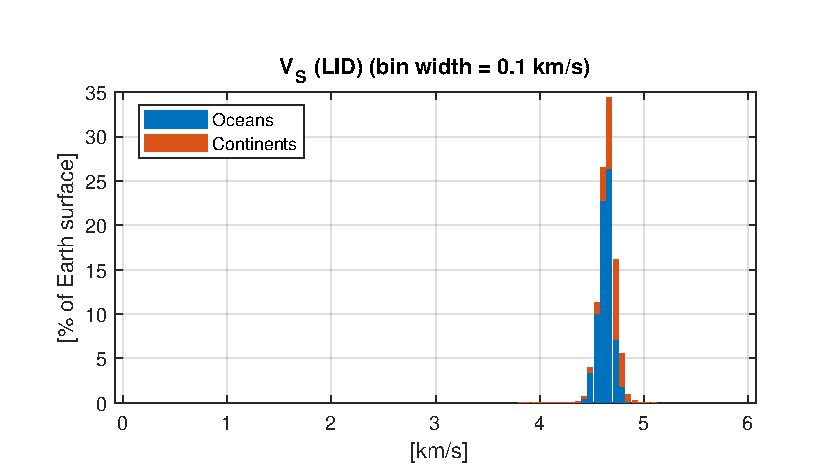
\includegraphics[width=\textwidth]{maps/sig_isol/VSLID.pdf} \\
                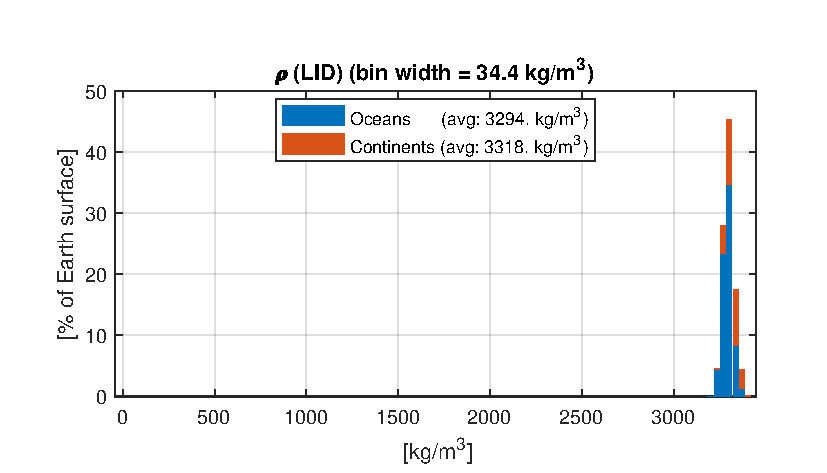
\includegraphics[width=\textwidth]{maps/sig_isol/RhoLID.pdf}
            \end{tabular}
        }
    \end{adjustbox}
    \caption[Density in the lithospheric mantle (LID) after conversion.]{
        \textbf{Top:}~shear wave velocity ($V_S$) in the lithospheric mantle (LID), from {LITHO1.0}. 
        \textbf{Bottom:}~lithospheric mantle average (bulk) density, obtained by velocity to density conversion.}
    \label{fig:SigIs:LID_VS-density_map}
\end{figure}

It must be noted that this conversion strategy was set up to enable propagation of lithospheric mantle inhomogeneities, as sensed by a model that provides only velocities.
I deemed a constant velocity-to-density scaling factor as an excessive simplification, since it would have ignored the lateral variations due to tectonothermal ages and the radial ones due to pressure dependence.
Still, since the main objective of these experiments is to assess an uncertainty modelling method, comprehensive thermochemical modelling was left out.

\subsection{Reference densities: layered normal Earth}
\label{ss:SigIs:InModels:REF}

As described in section~\ref{ss:SigIs:Defs:NETC}, the attraction of `anomalous masses' inside the planet is defined against the normal gravity  (Eq.~\ref{eq:red:Vdec2} and following).
By assuming that the normal gravity arises from a `reference Earth' with ellipsoidal stratification and with no lateral inhomogeneities, we can express any density refinement to the normal gravity model as a contrast against this `normal density reference'.
As mentioned in section~\ref{ss:SigIs:Defs:Corrs} and as discussed by \textcite{Vajda2008}, this should be satisfactorily approximated by reference earth models. \nocite{Moritz1990} \nocite{Tscherning1981} % probably I am citing these elsewhere
%The densities of the modelled layers are therefore expressed as density contrasts against a reference.

% slicing description
For all the sub-topography (i.e. sediments to lithospheric mantle) forward modelling performed here, a `normal density reference' was built, defined by a discretely layered reference column.
The boundaries between layers in this column define a set of concentric shells with constant depth against the reference ellipsoid.
The modelled layers in {LITHO1.0} were `sliced' according to these shells: in other words, an intersection was performed between the top/bottom boundaries defining each {LITHO1.0} layer and the reference shells boundaries (see Fig.~\ref{fig:SigIs:RefSlices}).
By doing so, each layer of the input model was divided in a number of \textit{layer-slices} equal to the number of reference shells it intersects.
In each layer-slice the density contrast was expressed as the difference between the density prescribed by the model at those coordinates and the density of the reference shell covering that depth range.

In order to build a reference density column, the density in each reference shell was computed by globally averaging the densities in the input model in the depth range defined by the shell.
Averages were weighted for the portion of shell occupied by each layer of the model (e.g. if in a specific grid node, in the \num{10} to \SI{18}{km} depth range, the first kilometre is occupied by the layer `SEDS3' and the remainder by `CRUST1', the average density is computed accordingly) and for the cosine of the latitude of each grid node (to account for the convergence of parallels in a regular grid, in a spherical approximation).

The maximum modelled depth was set to set to \SI{410}{\kilo \metre}, to account for the thickest lithosphere in {LITHO1.0}, \SI{320}{\kilo \metre} and a buffer for any additional depth introduced by the uncertainty-modelling perturbations.
The volume between the bottom of the lithosphere and the maximum modelled depth was filled-in with a `reference asthenosphere' with a density of \SI{3300}{\kilo \gram \per \cubic \metre}.
This a reference value which, albeit plausible \parencite[e.g.][]{Bormann2002}, is not directly constrained by the input data in any way - it is akin to the usual \SI{2670}{\kilo \gram \per \cubic \metre} adopted for the terrain correction \parencite{Hinze2003}.
As discussed afterwards (section~\ref{ss:SigIs:Results:Discussion}), any unmodelled sub-lithospheric density variation shows up in the refined gravity residuals (superimposed with all the omissions in the input `known masses' of the lithosphere).

The `normal density reference' obtained in this way ({LITHO1.0} densities and `asthenosphere fill-in') is presented in Fig.~\ref{fig:SigIs:Ref_ak135} (black line) and in Tab.~\ref{tab:Ref_ak135}.
The depth-density curve from the \textit{ak135} model \parencites{Kennett1995_ak135}{Montagner1996} is plotted alongside (blue line, the data was sourced from the {NMSOP-2} manual \cite{Bormann2002}, which provides it in a tabular form).
The \textit{ak135} model is also plotted as the average density in the same discrete depth intervals of the LITHO1.0-based density reference.

The density reference built using the {LITHO1.0} densities is considerably lower than \textit{ak135}, especially in the \num{18} to \SI{210}{\kilo \metre} depth range.
This arises from both omissions in the model and the constant \SI{3300}{\kilo \gram \per \cubic \metre} `asthenosphere fill-in' -- if \textit{ak135} was used as a fill-in instead, areas of thin lithosphere would contribute in raising the average.
Nevertheless, this strategy was preferred since, by doing so, the gravity maps of forward modelled masses (in terms of contrast) and the GGM with applied reductions are not overwhelmed by the signal of thickened lower density crustal keels reaching in an high density upper asthenosphere resulting from \textit{ak135} global average, which is sensibly biased by the predominance of oceanic lithosphere in the Earth. 

\begin{figure}
    \begin{adjustbox}{center}
        \fbox{
            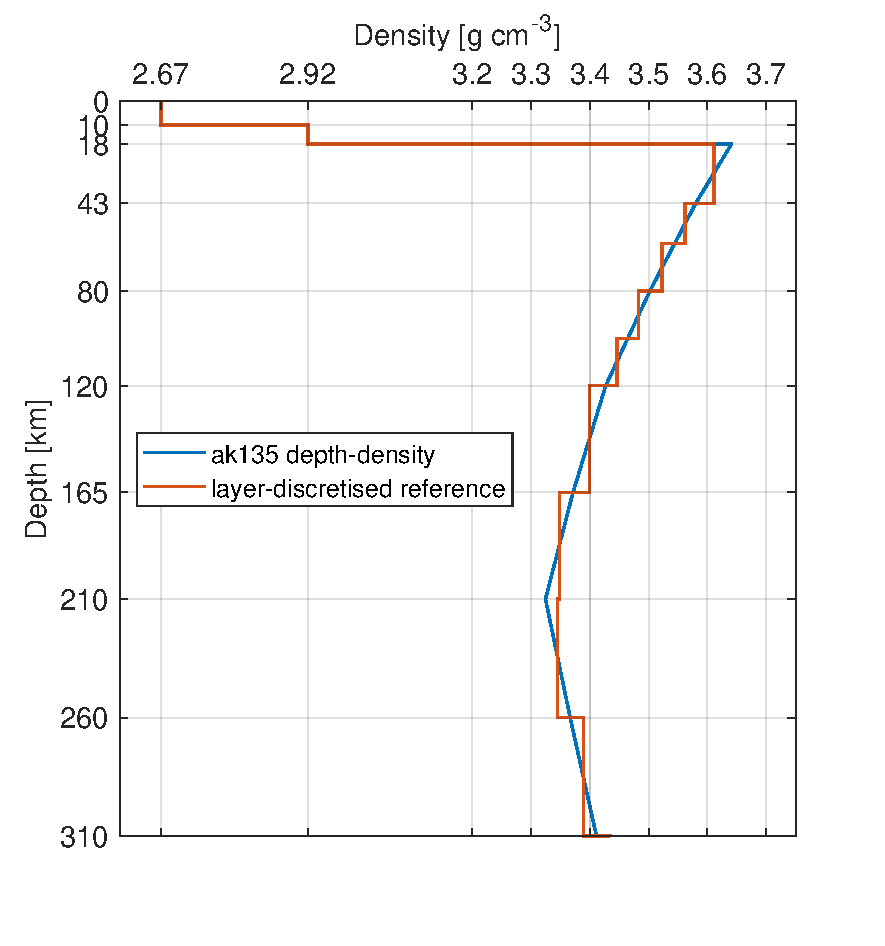
\includegraphics[
                width=0.75\textwidth,
                clip, trim=0.25cm 1.25cm 1.25cm 0cm
                ]{VSconv/ak135_RefCol.pdf}
        }
    \end{adjustbox}
    \caption[Depths and densities from the \textit{ak135} reference model, original,layer-discretised and computed on {LITHO1.0} data.]{
        \textbf{Blue}:~input depths and densities from the \textit{ak135} Earth reference model \parencite{Kennett1995_ak135}, set at \SI{2.67}{\gram \per \cubic \centi \metre} at less than \SI{10}{\kilo \metre}.
        \textbf{Orange}:~constant density reference layers obtained by averaging the \textit{ak135} model in discrete depth intervals.
        \textbf{Black}:~constant density reference layers obtained by averaging the \textit{LITHO1.0} \parencite{Pasyanos2014} model in the same discrete depth intervals of the orange curve.
        The layer-discretised densities are shown in Tab.~\ref{tab:Ref_ak135}.}
    \label{fig:SigIs:Ref_ak135}
\end{figure}

\begin{table}
    \caption[AAA]{Average densities of the \textit{ak135} Earth reference model, obtained by interpolation in discrete depth intervals, and average densities derived from the \textit{LITHO1.0} global data, computed inside the same depth intervals).
    See also Fig.~\ref{fig:SigIs:Ref_ak135}.}
    \begin{adjustbox}{center}
        \begingroup\setlength{\fboxsep}{0pt}
        \colorbox{tablebackground}{%
        \begin{tabular}{rll}
            \toprule
            \multicolumn{1}{c}{\textbf{Depth}} & \multicolumn{2}{c}{\textbf{Density}} \\
            \multicolumn{1}{c}{\textbf{[\si{\kilo \metre}]}} & \multicolumn{2}{c}{\textbf{[\si{\gram \per \cubic \centi \metre}]}} \\
            \midrule
            & \multicolumn{1}{c}{\textit{ak135}} & \multicolumn{1}{c}{\textit{LITHO1.0}} \\
            \midrule
            0   & \multirow{2}{*}{2.670} & \multirow{2}{*}{2.670} \\
            10  & \multirow{2}{*}{2.920} & \multirow{2}{*}{2.968} \\
            18  & \multirow{2}{*}{3.631} & \multirow{2}{*}{3.111} \\
            26  & \multirow{2}{*}{3.611} & \multirow{2}{*}{3.162} \\
            35  & \multirow{2}{*}{3.590} & \multirow{2}{*}{3.214} \\
            43  & \multirow{2}{*}{3.562} & \multirow{2}{*}{3.279} \\
            60  & \multirow{2}{*}{3.523} & \multirow{2}{*}{3.301} \\
            80  & \multirow{2}{*}{3.483} & \multirow{2}{*}{3.307} \\
            100 & \multirow{2}{*}{3.446} & \multirow{2}{*}{3.310} \\
            120 & \multirow{2}{*}{3.399} & \multirow{2}{*}{3.311} \\
            165 & \multirow{2}{*}{3.348} & \multirow{2}{*}{3.311} \\
            210 & \multirow{2}{*}{3.345} & \multirow{2}{*}{3.308} \\
            260 & \multirow{2}{*}{3.389} & \multirow{2}{*}{3.301} \\
            310 \\
            \bottomrule
        \end{tabular}}
        \endgroup 
    \end{adjustbox}
    \label{tab:Ref_ak135}
\end{table}

\begin{figure}
    \begin{adjustbox}{center}
        \fbox{
            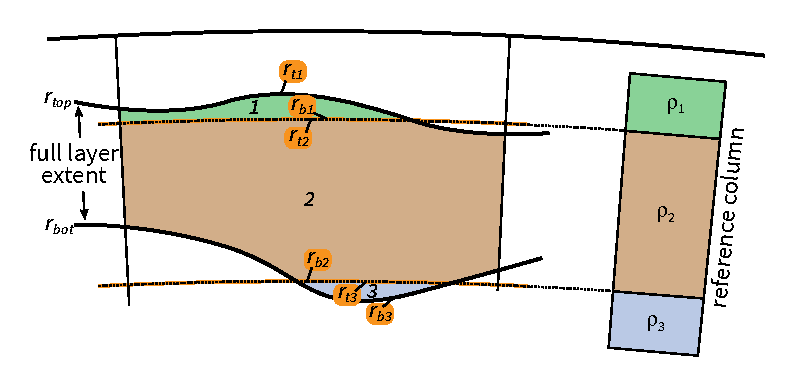
\includegraphics[width=\textwidth]{forward_layer_slice_out.pdf}
        }
    \end{adjustbox}
    \caption[Sketch describing the `slicing' of layers according to a reference density model.]{
        Sketch describing the `slicing' of layers according to a reference density model (a concentric depthwise succession of constant density shells).
        The input, non-partitioned, layer is defined by top and bottom surfaces $r_{top}$ and $r_{bot}$, expressed as radius.
        The portion of layer in the $i$-th reference shell is expressed as separate top and bottom sub-surfaces $r_{ti}$ and $r_{bi}$.
        Where no part of the layer interesects a reference shell, i.e. where there is no mass to model, the two surfaces coincide.}
    \label{fig:SigIs:RefSlices}
\end{figure}

\FloatBarrier

\section{Assessment of uncertainty}
\label{s:SigIs:Impl}

Uncertainty in the `known masses' input data was estimated using Monte Carlo error propagation \parencite[][chapter 2.6]{Aster2018}.
Depths of the boundaries, defining the layers in {LITHO1.0}, and the density grids associated with each layer were randomly perturbed according to a set of error assumptions, obtaining a population of input mass models.
The gravity field of each of this mass models was forward modelled using the spectral layer-wise method described in this chapter, therefore obtaining a population of resulting gravity fields.
To extract a metric of the spatial distribution of uncertainty and its magnitude, I then computed the standard deviation of the vertical component of gravity at each grid node of the ensemble of globally synthesized grids.

As described in section~\ref{ss:SigIs:LITHOmodel}, {LITHO1.0} is provided with no information on uncertainty, nor on the spatial variability of data resolution.
At the time of setting up and running this uncertainty assessment, the only crustal scale models providing error information where regional extent Moho depth models: e.g.~\textcite{Grad2009} and \textcite{Artemieva2013} for the European plate, \textcite{Steffen2017} in Greenland, \textcite{VanderMeijde2013} in South America, to name a few.
% posso ricavare valori plausibili da moho globali
% eshagh e GEMMA (leggo bene, diverso modo uncertainty)
% così giustifico i miei valori
% e cito valori Szwillus (2019) per lo stesso motivo

% multiprocessing

% spostati commenti seguenti da FWD
% razionale per il metodo: random modelling

% razionale per il numero di campioni: euristica, needs further validation for efficient use of computational resources


\FloatBarrier

\section{Global reduction results}
\label{s:SigIs:Results}



\subsection{Spectral domain comparison}
\label{ss:SigIs:Results:Spectral}

\subsection{Discussion}
\label{ss:SigIs:Results:Discussion}
% confronto con tenzer2009 (e 2015)
% statico-no-uncertainty
% a strati (con ancora segnale ondulazione)
% vs "a gusci"
% esempio taglio a massima profondità Moho
% v. appunti 20190821

% considerazioni su input bandwidth: sposto a discussione
% for in detail, reader is referred to Hirt and Kuhn 2017
% "While the topography mass models are strictly band-limited to the NT max values reported in Table 1, the topography-implied gravity contains signals at harmonic degrees much larger than NT max" [Hirt and Kuhn, 2014]

% questioni isostatiche: summary and conclusions Sebera 2018
% ricordarsi che Sebera 2018 non è reductions, è forward assoluto (no contrasti)


% SCELTA REFERENCE, differenza è media (circa media)
% note su rilevanza densità media
%reference density in a spherical shell
% slightly more complex for ell, stops at degree
% cito... Hirt and Rexer? fino a che grado
% 
%therefore a wrong reference
%of the average
%or a reasonable approximation of the average
% noto che media può essere utilizzata per ri-definire valore medio
% out of scope of these experiments
%
% CRUST-MANTLE a 18 km (media globale ak135) è molto sottile per continenti!
% fwd con ak135 come fill in: sebera2014

% altro appunto su ref densities: a cosa corrispondono ref densities da ak135 nelle conversioni Rho(VS, P)?

% questioni numeriche: pag. 24 di Root (2015)
% faccio doppio calcolo per coefficienti (con sovrapposizione)
% di contro, rispetto a Novak, faccio singolo rho*h in spatial domain
% risparmiandomi una GSHA (SH analysis grid->SH), che è expensive
% implementazione nello script: GSHA per interfacce fatta il doppio
% perché ne faccio una sia per il bottom dello strato sopra
% che per il top dello strato sotto

% "è necessario rimuovere segnale litosferico?"
% esistono approcci alternativi: Greff-Lefftz 2016, Panet 2014 - giustificato da Ricard 2006
% con questo mostro un esempio: solo gradi bassi vs rimozione litosfera (ai gradi bassi)

\begin{subappendices}
\section[Supplementary:~testing the method against spatial--domain forward modelling]{Supplementary: testing the method against spatial--domain forward modelling}
\label{s:SigIs:Test}

Modelling setups such as the one employed in this chapter are commonplace, with different technical choices being dictated by application requirements.
However, I decided to supplement these modelling experiments with a set of direct comparison tests aimed to assess:
1) the behaviour of the layer--wise modelling (section~\ref{ss:SigIs:Fwd:LayerFwd}), since it is an ``off-label'' use of the single-relief forward modelling method by \textcite{Wieczorek2007};
2) the difference in results against a spatial domain modelling method, given the well known issues with limited bandwidth of spectral domain methods \parencite{Hirt2014}.

A rigorous assessment of the convergence of the layer--wise arrangement adopted in this work is not available at the moment.
Therefore, an heuristic test was devised to assess if such a strategy was fit for these experiments purpose, i.e. \si{\milli Gal} level accuracy at comparatively low degrees (limited by satellite-only gravity models).
As it is shown later, the satisfactory results of the direct comparison and the larger magnitude of the contribution of uncertainty of geophysical models were enough to support leaving any more rigorous analysis to further development.

\subsection{Synthetic model: ``four blocks test''}
\label{ss:SigIs:Test:FourBlocks}

A synthetic mass distribution was defined, made up of four 2$\times$2~degree ``blocks'', each \SI{1}{\kilo \metre} thick.
Set on a sphere with radius equal to WGS84 semi-major axis (\SI{6378.137}{\kilo \metre}), two blocks rise above it, the remaining two below it, arranged in a checkerboard fashion.
The bodies above the sphere radius have a density of $+$\SI{1}{\gram \per \cubic \centi \metre}, those below have a density of \SI{-1}{\gram \per \cubic \centi \metre}.
The resulting relief map is plotted in Fig.~\ref{fig:SpatSpecComp:4B_DepthMap}, zoomed in on the area covered by the blocks (centered on \SI{47}{\degree N}, \SI{47}{\degree E}).
The grid covers the whole globe and contains no other masses.
Owing to the limited bandwidth requirement of the input grids for the spectral method (section~\ref{ss:SigIs:Fwd:SHtransform}), the original square-wave shaped relief map was low-pass filtered with a Gaussian kernel ($e^{-1/2}$ response at \SI{4}{\degree}).
All the three forward modelling methods tested employ a \SI{0.0625}{\degree}$\times$\SI{0.0625}{\degree} equally spaced global grid.

A section along the \SI{48}{\degree N} parallel is plotted in Fig.~\ref{fig:SpatSpecComp:4B_sections}, which shows the three ways in which the mass distributions have been expressd:
\begin{enumerate}
\item[a)] \textbf{one relief}, input for the unmodified spectral-domain method of \textcite{Wieczorek2007}. The reference sphere radius $D$ is set equal to the zero-relief sphere radius (\SI{6378.137}{\kilo \metre}). The input density is set uniform everywhere: its effect is negative in areas with negative relief, due to the $\rho h$ product (Eq.~\ref{eq:SHfwd:reliefSH}).
\item[b)] \textbf{layer-wise} setup: positive- and negative-relief volumes are modelled as two separate layers. The reference sphere radius $D$ is set equal to the highest relief. The aforementioned zero-relief sphere serves as the bottom boundary for the positive relief layer and as the top boundary for the negative relief one. Input density is positive above zero (red fill) and negative below (blue fill) -- as mentioned in the strategy description, density signs are then reversed in the forward-modelling function, since height in respect to $D$ is negative.
\item[c)] spatial-domain \textbf{tesseroids} discretisation: the relief was turned into discrete spherical tesseroids, sized with the same grid spacing as the input grid and centered on the grid nodes (\textit{grid registration}). Forward modelling was carried out with the Tesseroids code \parencites{Uieda2016}{UiedaTesseroids}.
\end{enumerate}

\begin{figure} % 4 blocks, depth map
    \begin{adjustbox}{center}
        \fbox{
            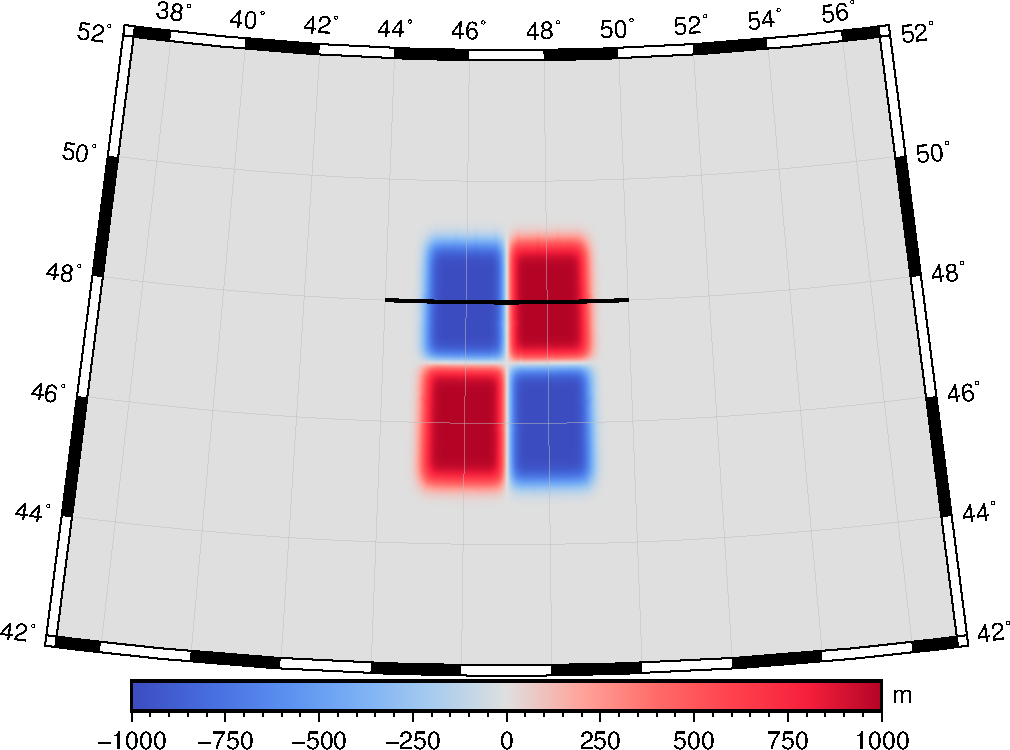
\includegraphics[width=0.9\textwidth]{maps/spatial_spectral_comparison/BLO_depth.pdf}
        }
    \end{adjustbox}
    \caption[Relief map of the synthetic mass distribution used to compare the three modelling methods.]{
        Relief map of the synthetic mass distribution (``four blocks test'') used to compare the three modelling methods.
        Heights (and depths) are expressed in respect to a reference sphere with radius equal to \SI{6378.137}{\kilo \metre} (semi-major axis of {WGS84}).
        The black line along the \SI{48}{\degree N} parallel denotes the profile shown in Fig.~\ref{fig:SpatSpecComp:4B_sections}.}
    \label{fig:SpatSpecComp:4B_DepthMap}
\end{figure}

\begin{figure} % 4 blocks, sections
    \begin{adjustbox}{center}
        \fbox{
            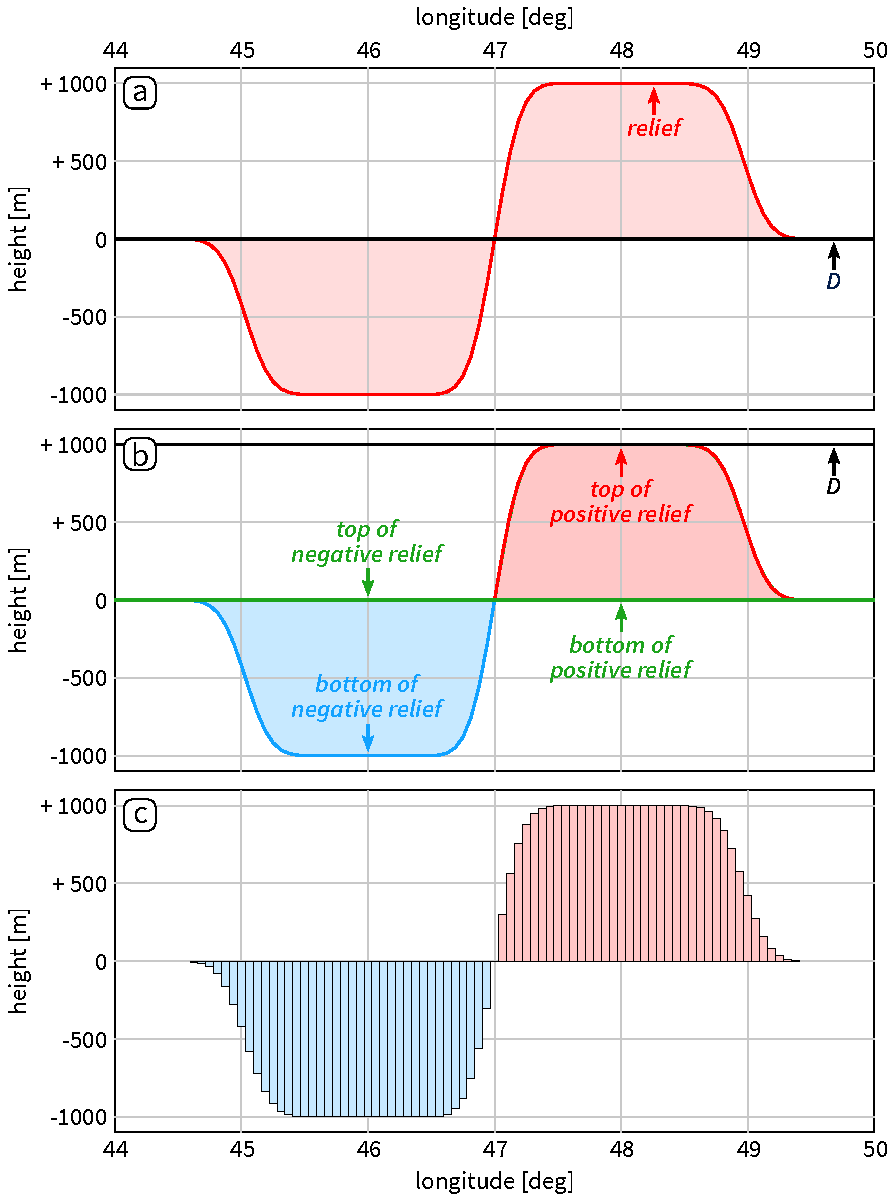
\includegraphics[width=0.9\textwidth]{tess_test/tess_test_ElevPlot_stairs_mod_out.pdf}
        }
    \end{adjustbox}
    \caption[Sections trough the synthetic mass distribution in the three tested modelling methods]{
        Sections trough the synthetic mass distribution (Fig.~\ref{fig:SpatSpecComp:4B_DepthMap}) in the three tested methods:
        \textbf{a)}~one relief against a reference sphere of radius $\bm{D}$, input for the unmodified spectral-domain method of \textcite{Wieczorek2007};
        \textbf{b)}~the layer-wise spectral-domain strategy adopted in this chapter: two separate layers for the positive and negative density volumes, each defined by a top and bottom surface, and a common reference sphere;
        \textbf{c)}~tesseroids discretisation (\SI{0.0625}{\degree}$\times$\SI{0.0625}{\degree}), input for the spatial-domain method \parencite{Uieda2016}.
        All heights are expressed in respect to a reference sphere with radius equal to \SI{6378}{\kilo \metre}.
        The red-filled areas denote positive input densities ($+$\SI{1}{\gram \per \cubic \centi \metre}) and the blue-filled ones denote negative input densities (\SI{-1}{\gram \per \cubic \centi \metre}).}
    \label{fig:SpatSpecComp:4B_sections}
\end{figure}

\paragraph*{Four blocks test, $g_z$ grids}
Figure~\ref{fig:SpatSpecComp:4B_g_maps} shows the results and direct comparison between spectral-domain (method \textbf{a)}) and spatial-domain (method \textbf{c)}).
The difference between the spectral and spatial output (spatial minus spectral $g_z$, lower left panel) lies inside a \num{-0.92} to \SI{0.92}{\milli Gal} range.
It is affected by the characteristic side lobes (\textit{ringing}) which arise due to the boxcar truncation of the spherical harmonic expansion \parencite{BarthelmesGentleCut2008}.
Applying a linerly decreasing weight (from 1 to 0) to all coefficients from degree 200 to 360 results in the differences plotted in the lower right panel.
This \textit{gentle cut} truncation was applied both to the coefficients resulting from the spectral method and to the results of Tesseroids modelling, by transforming the global grids in a spherical harmonics expansion, applying the truncation and synthesizing $g_z$.
The filtered $\Delta g_z$ is distributed between \num{-0.0184} and \SI{0.0181}{\milli Gal}.

\begin{figure} % 4 blocks, output maps
    \begin{adjustbox}{center}
        \fbox{
            \begin{tabular}{cc}
                \begin{overpic}[width=0.65\textwidth]{maps/spatial_spectral_comparison/BLO_S.pdf}
                    \put (15,62.5) {\large \textsf{\textbf{$\bm{g_z}$, spectral}}}
                \end{overpic} &
                \begin{overpic}[width=0.65\textwidth]{maps/spatial_spectral_comparison/BLO_T.pdf}
                    \put (15,62.5) {\large \textsf{\textbf{$\bm{g_z}$, spatial}}}
                \end{overpic} \\
                \begin{overpic}[width=0.65\textwidth]{maps/spatial_spectral_comparison/BLO_D.pdf}
                    \put (15,62.5) {\large \textsf{\textbf{$\bm{\Delta g_z}$, boxcar truncation}}}
                \end{overpic} &
                \begin{overpic}[width=0.65\textwidth]{maps/spatial_spectral_comparison/BLO_Dt.pdf}
                    \put (15,62.5) {\large \textsf{\textbf{$\bm{\Delta g_z}$, tapered truncation}}}
                \end{overpic}
            \end{tabular}
        }
    \end{adjustbox}
    \caption[Forward modelled output of the spectral--spatial comparison, ``four blocks test''.]{
        Forward modelled output of the spectral--spatial comparison, ``four blocks test''.
        These four maps show the radial component $g_z$ of the attraction of the modelled masses, expressed as positive upwards (i.e. a positive density contrast result in a negative $g_z$ directly above it).
        The observation height is \SI{40}{km} above the reference sphere.
        The two maps on bottom row show the spatial minus spectral $g_z$ difference.
        In the lower left map, the spherical harmonics coefficients were synthesized up to degree and order $l_{max}$ \num{360}, with an abrupt truncation at $l_{max}$.
        In the lower right map, a linear taper was applied to the coefficients above degree \num{200}, reaching zero weight at $l_{max}$.
    }
    \label{fig:SpatSpecComp:4B_g_maps}
\end{figure}

\begin{figure} % 4 blocks, deg var spectra comparison: layers vs tesseroids
    \begin{adjustbox}{center}
        \fbox{
            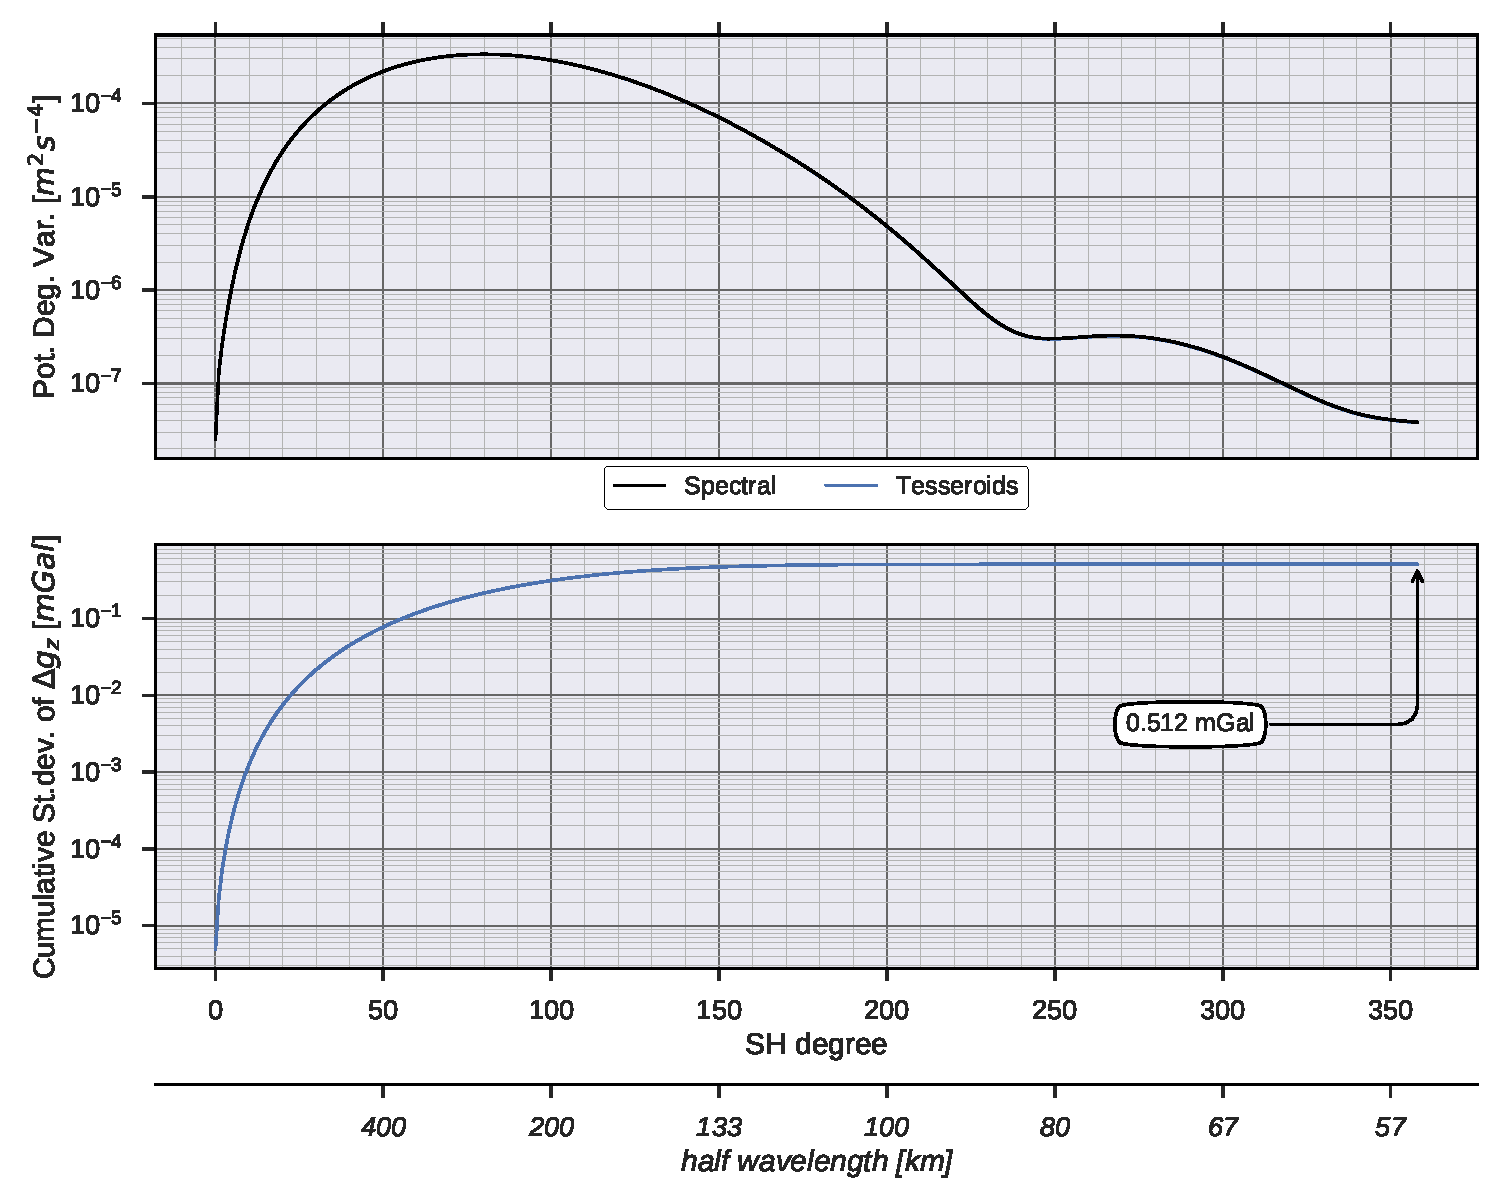
\includegraphics[width=1.2\textwidth]{tess_test/FwdTest_degvar_comp.pdf}
        }
    \end{adjustbox}
    \caption[Spectral domain modelling against spatial domain modelling: degree variance and difference spectra (four blocks test).]{
        Spectral domain (layer-wise) modelling against spatial domain (Tesseroids) modelling: degree variance and difference spectra for the ``four blocks test''.
        The \textbf{upper panel} shows the degree variance power spectra of the forward-modelled potential of the two methods.
        Note that no difference can be graphically appreciated between the two plotted curves.
        The \textbf{lower panel} show the cumulative standard deviation spectra of the differences in radial component of gravity ($g_z$), computed as spatial-domain minus spectral-domain.}
    \label{fig:SpatSpecComp:4B_dv_spec_tess}
\end{figure}

\paragraph*{Four blocks test, power spectrum}
The same output can be expressed in the spectral domain, by comparing the power spectra of the modelled fields. The upper panel of Fig.~\ref{fig:SpatSpecComp:4B_dv_spec_tess} shows the degree variances (Eq.~\ref{eq:DegVar}) of the potentials obtained with the spectral-domain method and with the spatial-domain one (after transforming the global grid in spherical harmonics).
To better express the differences (spatial minus spectral), which are not evident in the degree variances plot, the spectrum of the standard deviation of $\Delta g_z$ is shown in the bottom panel of the same figure.
This spectrum was also obtained by prior spherical harmonics expansion of the synthesized $g_z$ grids, unfiltered (no \textit{gentle cut} applied).
It is expressed cumulatively, reaching a maximum of \SI{0.512}{\milli Gal} at $l_{max}$.

\begin{figure} % 4 blocks, deg var spectra comparison: 1 relief vs layers
    \begin{adjustbox}{center}
        \fbox{
            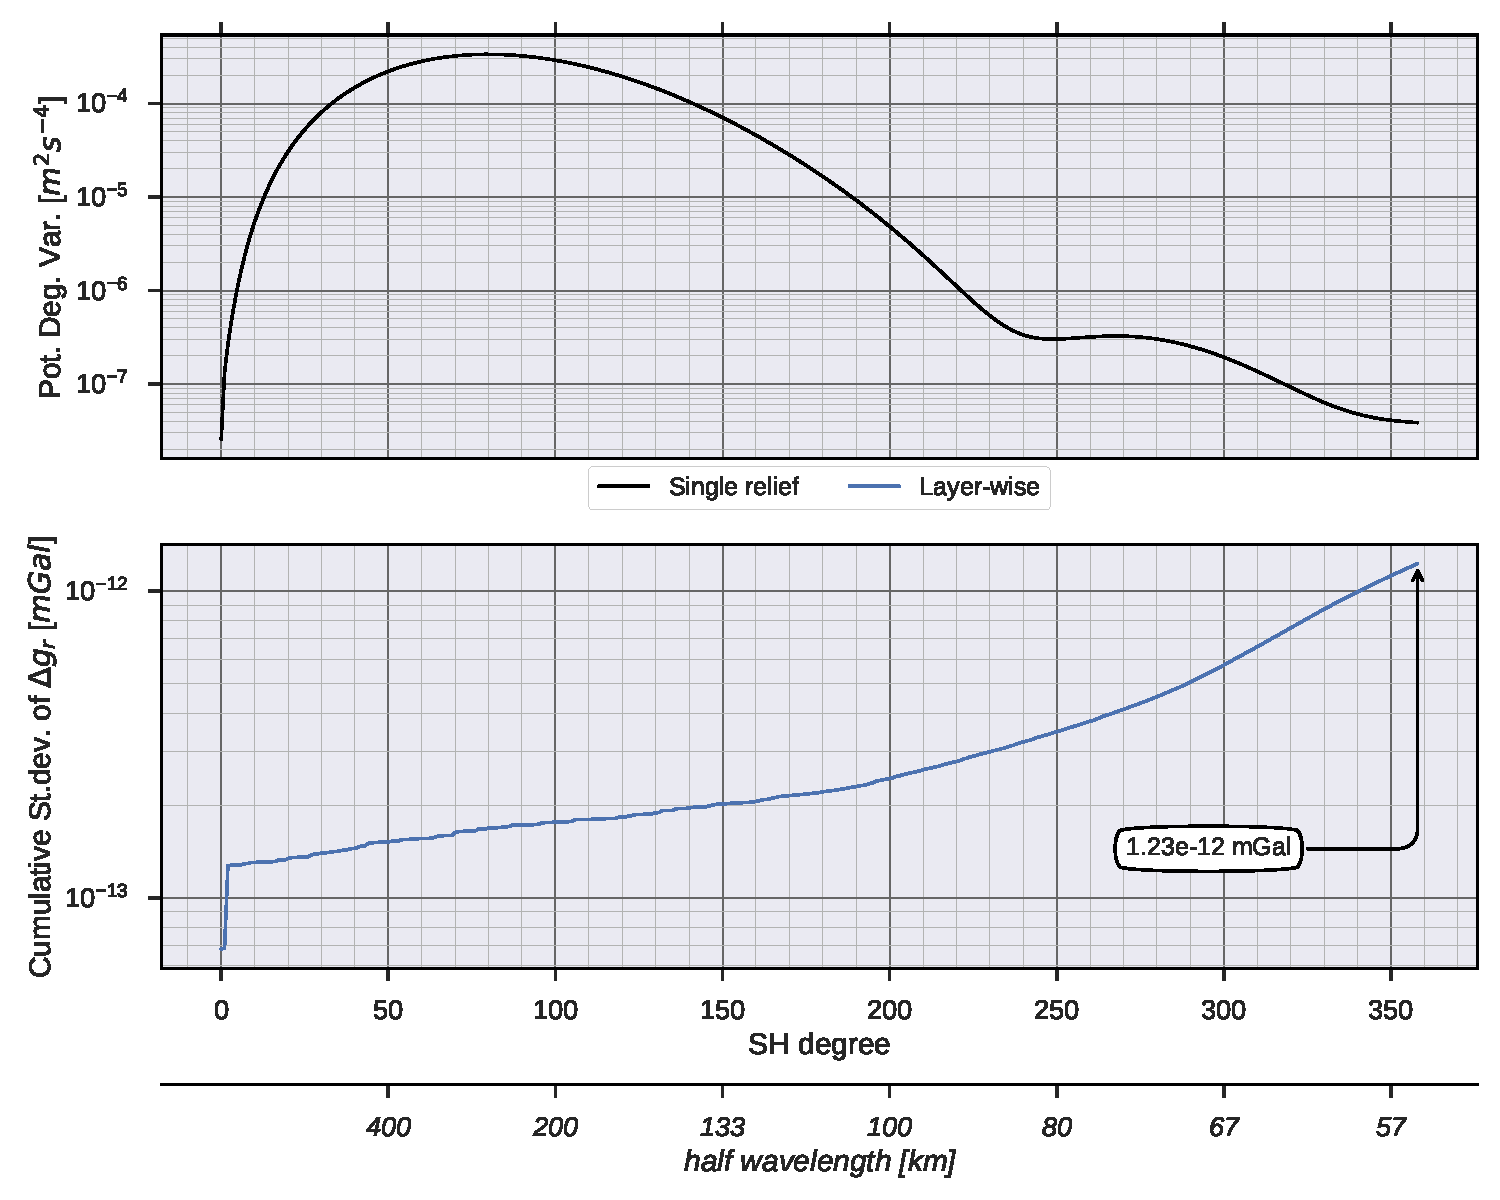
\includegraphics[width=1.2\textwidth]{tess_test/FwdTest_degvar_spec_comp.pdf}
        }
    \end{adjustbox}
    \caption[``Single-relief'' against layer-wise comparison: degree variance and difference spectra.]{
        ``Single-relief'' against layer-wise comparison: degree variance and difference spectra.
        The \textbf{upper panel} shows the degree variance power spectra of the potential resulting from the ``four blocks test'' in the single-relief setup \parencite[unmodified method of][]{Wieczorek2007} and in the layer-wise strategy adopted in this chapter.
        The differences in input-masses representation between the two methods are shown in Fig.~\ref{fig:SpatSpecComp:4B_sections}.
        Note that no difference can be graphically appreciated between the two plotted curves.
        The \textbf{lower panel} show the cumulative standard deviation spectra of the differences in radial component of gravity ($g_z$), computed as layer-wise minus single-relief.}
    \label{fig:SpatSpecComp:4B_dv_spec_relief}
\end{figure}

\paragraph*{Four blocks test, single relief against layer-wise method}
In addition to the spectral-domain (method \textbf{a)}) against spatial-domain (method \textbf{c)}) comparison, the consistency between two spectra-domain methods was tested: the unmodified relief-forward-modelling of \textcite{Wieczorek2007} (method \textbf{a)}) and its implementation as a layer-wise approach (method \textbf{b)}).
The results, expressed in terms of power spectra (degree variances of the potential) and spectrum of $g_z$ differences (cumulative degreee standard deviation) are shown in Fig.~\ref{fig:SpatSpecComp:4B_dv_spec_relief}.
The two strategies converge to identical results, the only discrepancy likely arising from computational precision.
Cumulative standard deviation of $\Delta g_z$ at $l_{max}$ is \SI{1.23e-12}{\milli Gal}.

\subsection{Test using the SEDS1 layer}
\label{ss:SigIs:Test:SEDS1}

I am also including the output of another test: instead of the ``synthetic relief'' just shown in section~\ref{ss:SigIs:Test:FourBlocks}, here the real layer boundaries of a layer from LITHO1.0 \parencite{Pasyanos2014} was used, representing a real step of the forward modelling carried out in this chapter.
The {SEDS1} layer is the most superficial among the layer modelled here (see the general model description in section~\ref{ss:SigIs:LITHOmodel}).
Representing the first of three sedimentary layers, it is derived from an updated version of the global sediment thickness map by \textcite{Laske1997_sediments}.
The only difference with the modelled reductions (section \ref{s:SigIs:Results}) is that the prescribed depths were referred to a sphere (instead of the WGS84 ellipsoid), the observation points were also spherical (\SI{40}{\kilo \metre} above the sphere) and density has been imposed constant at \SI{2.17}{\gram \per \cubic \centi \metre} (modelled as a \SI{-0.50}{\gram \per \cubic \centi \metre} contrast against a \SI{2.17}{\gram \per \cubic \centi \metre} reference density).
These three modifications simplified the generation of the corresponding tesseroids-discretised model and computation points grid, thus avoiding a potential source of discrepance in the direct comparison.

The direct comparison on synthesized $g_z$ maps is shown in Fig.~\ref{fig:SpatSpecComp:SEDS1_g_maps}.
Differences, expressed as Tesseroids-modelled $g_z$ minus spectral-domain layer-wise modelled $g_z$, are shown in the lower map.
They are distributed between \num{-0.099} and \SI{0.129}{\milli Gal}, with local maxima concentrating on margin areas -- likely arising from issues in correctly modelling sharp edges with the limited bandwidth of the spectral method.
The range of the difference expressed in relative terms (as percentage of the signal at the same point) is \SI{-0.448}{\percent} to \SI{0.345}{\percent}.
In regards to the maximum power ($n_{max}$) in the relief spherical harmonics expansion (Eq.~\ref{eq:SHfwd:coeffs}), values ranging from \num{2} to \num{14} were tested, observing no significant change in spectral-to-spatial differences.
Owing to the short time requirements for a single spectral forward modelling run, a mid-range $n_{max}$ of 7 was chosen (the run times for $n_{max}$ of 2, 7, 14 are \SI{2.2}{s}, \SI{4.2}{s}, \SI{6.1}{s} respectively).
The minimum and maximum difference are reported here for $n_{max}$ equal to 2 and 14, respectively: \num{-0.201} to \SI{0.212}{\milli Gal} and \num{-0.099} to \SI{0.129}{\milli Gal} (the former are identical to the min/max range at $n_{max}=\textrm{\num{7}}$).

\begin{figure} % SEDS1 test, output maps
    \begin{adjustbox}{center}
        \fbox{
            \begin{tabular}{cc}
                \begin{overpic}[width=0.65\textwidth]{maps/spatial_spectral_comparison/SED_St.pdf}
                    \put (0,62) {\large \textsf{\textbf{$\bm{g_z}$ S}}}
                \end{overpic} &
                \begin{overpic}[width=0.65\textwidth]{maps/spatial_spectral_comparison/SED_Tt.pdf}
                    \put (0,62) {\large \textsf{\textbf{$\bm{g_z}$ T}}}
                \end{overpic} \\
                \multicolumn{2}{c}{
                    \begin{overpic}[width=1.3\textwidth]{maps/spatial_spectral_comparison/SED_Dt.pdf}
                        \put (0,62) {\large \textsf{\textbf{$\bm{\Delta g_z (\textsf{T} - \textsf{S})}$}}}
                    \end{overpic}
                }
            \end{tabular}
        }
    \end{adjustbox}
    \caption[Spectral domain modelling against spatial domain modelling: SEDS1 test, direct comparison of $g_z$.]{Spectral domain (layer-wise) modelling against spatial domain (Tesseroids) modelling: direct comparison using the {SEDS1} layer from {LITHO1.0}.
    All the maps show the vertical (radial) component of $g$.
    Upper left map: spectral domain $g_z \ S$, upper right map: spatial domain $g_z \ T$, lower map: difference, expressed as spatial minus spectral.}
    \label{fig:SpatSpecComp:SEDS1_g_maps}
\end{figure}

\begin{figure} % SEDS1 test, deg var spectra comparison
    \begin{adjustbox}{center}
        \fbox{
            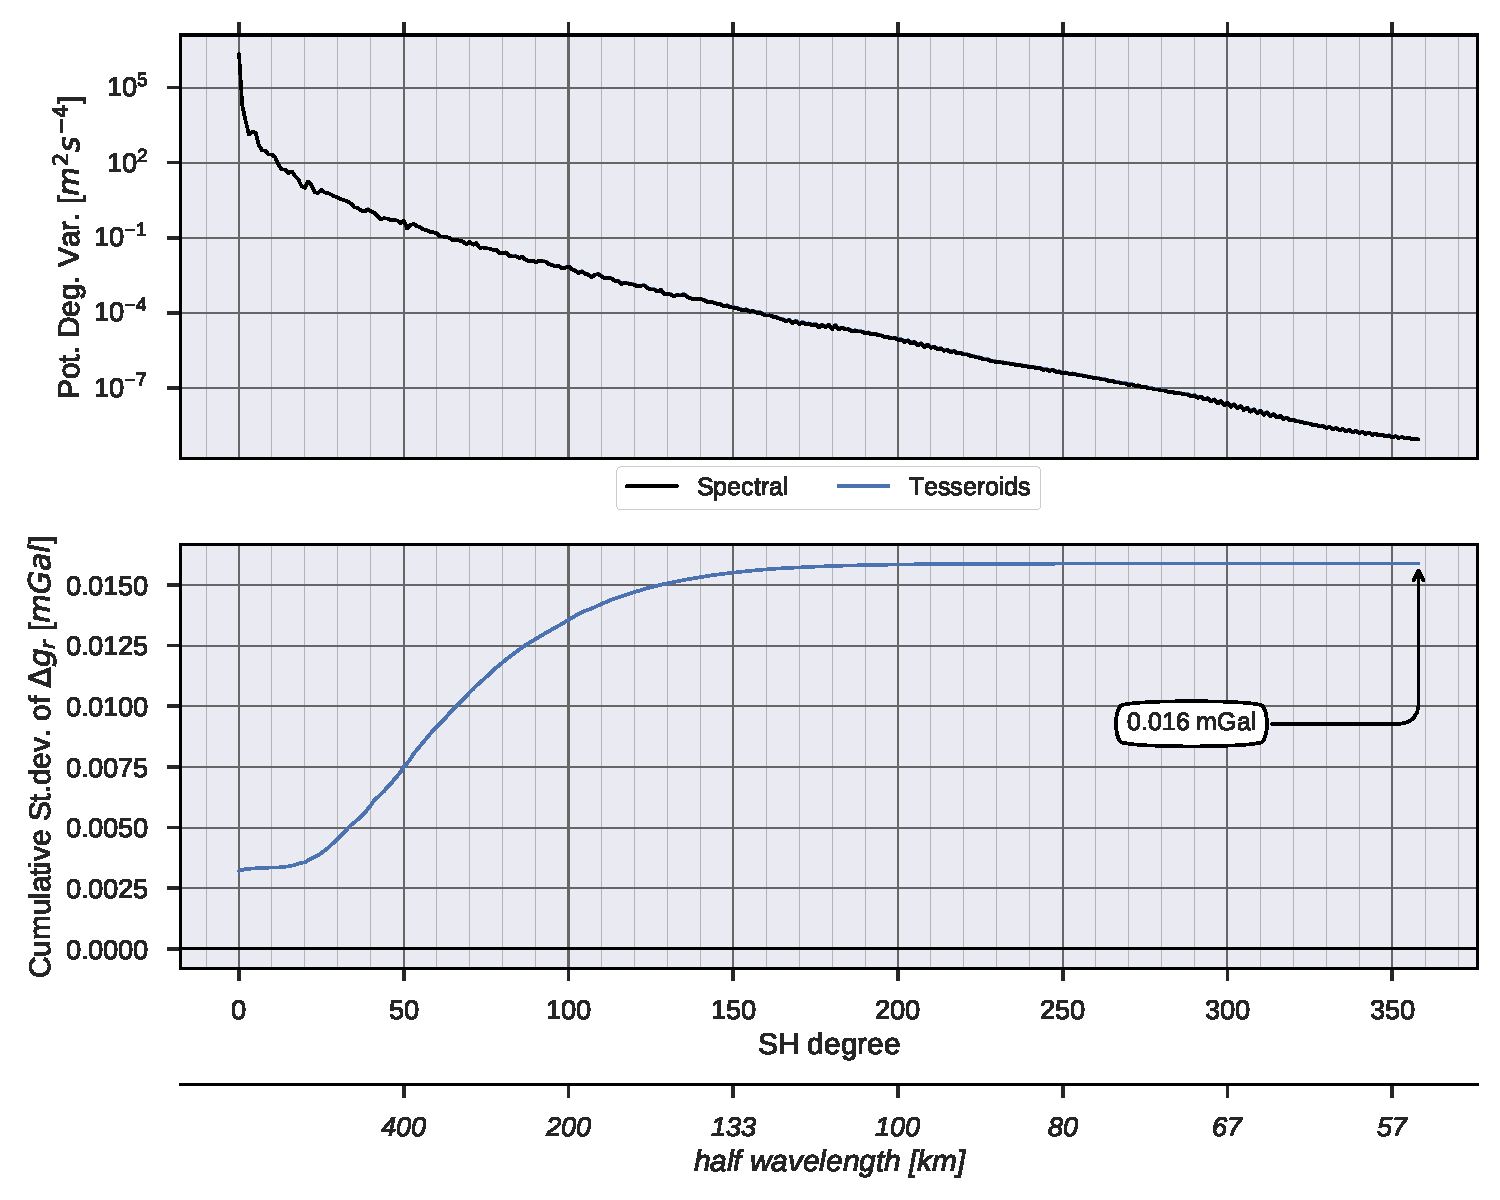
\includegraphics[width=1.2\textwidth]{tess_test/FwdTest_SEDS_degvar_comp.pdf}
        }
    \end{adjustbox}
    \caption[Spectral domain modelling against spatial domain modelling: degree variance and difference spectra (SEDS1 test).]{
        Spectral domain (layer-wise) modelling against spatial domain (Tesseroids) modelling: degree variance and difference spectra for the SEDS1 test (Fig.~\ref{fig:SpatSpecComp:SEDS1_g_maps}).
        The \textbf{upper panel} shows the degree variance power spectra of the forward-modelled potential of the two methods.
        Note that no difference can be graphically appreciated between the two plotted curves.
        The \textbf{lower panel} show the cumulative standard deviation spectra of the differences in radial component of gravity ($g_z$), computed as spatial-domain minus spectral-domain.
    }
    \label{fig:SpatSpecComp:SEDS1_dv_spec}
\end{figure}

Figure~\ref{fig:SpatSpecComp:SEDS1_dv_spec} shows the spectral- to spatial-domain comparison in terms of power spectra (upper panel) and cumulative standard deviation spectrum of the gravity ($g_z$) differences (lower panel).
The same process adopted for the ``four-block test'' was adopted here: in order to perform a spectral domain comparison, the spatial domain output was transformed in a spherical harmonics expansion.
Both plots show a satisfactory coherency.
The two potential degree variance curves are non-distinguishable and the $\Delta g_z$ spectrum plot, which amplifies the differences, show a misfit level in the order of magnitude of tens of \si{\micro Gal}.
The cumulative standard deviation of  $\Delta g_z$ at $l_{max}$ is \SI{0.016}{\milli Gal}.

%\subsection{Outcome of the tests}
%\label{ss:SigIs:Test:Outcome}

Overall, the two tests that were presented here show a satisfactory agreement between the spatial-domain method (adopted as a benchmark) and the layer-wise spectral-domain technique that was employed in computing the reductions and uncertainty-propagation of this chapter.
Misfit levels, both in a synthetic 2$\times$2 checkerboard test and with a realistic global layer, are small enough to exceed the application requirements: they lie below the uncertainties involved in the input mass distribution data.
In addition, the layer-wise spectra-domain modelling technique, which relies on the superposition of the effects of the top and bottom surfaces of a layer, was shown to provide identical results to the single relief modelling provided in SHTOOLS \parencite{Wieczorek2018}.

The direct comparison of spatial- and spectral-domain methods also allowed to quantify and compare the computational time requirements, which has been the rationale for preferring the faster spectral-domain method for the Monte Carlo uncertainty propagation.
For a single layer, provided on a global $n \times 2n$ grid with a \SI{0.25}{\degree} spacing, the spectral-domain method takes about 3~seconds, comprising two spherical harmonic transforms (for the top and bottom input reliefs), two calls to the forward-modelling routine, and a spectral harmonic synthesis to four output grids (the potential and the three components of its first derivative, $g$)
In order to obtain a similar result in space domain, using Tesseroids \parencite{UiedaTesseroids} on the same grid, a total number of \SI{1036800}{tesseroids}$\times$\SI{1036800}{computation points} must be calculated.
This requires a run time of about \SI{240}{hours}, which becomes feasible only by resorting to parallelisation -- the SEDS1 test was run on \num{100} parallel workers, requiring \SI{2.26}{hours}.

However, it must be noted that this remarkable difference in computational requirements and this spatial- to spectral-domain equivalence is true only in this peculiar configuration, given the requirements of these reduction experiments: relatively low-resolution input data, with a large associated uncertainty, and a relatively low-degree band-limited output requirement (the satellite-only global gravity models at which the reductions are aimed).
\end{subappendices}
